\documentclass[pdftex]{article}
\usepackage[]{geometry-commomun}

\hypersetup{%
  a4paper,
  colorlinks=true,
  filecolor=blue,
  linkcolor=brick,urlcolor=red,
  pdfstartview=Fit,
  pdfauthor={Olivier Guib�, Philippe Ivaldi},
  pdfsubject={Plane geometry with Asymptote},
  pdftitle={Plane geometry module for Asymptote},
  pdfkeywords={geometry , plane, software, module, package, extension, package,
    vector, latex, asymptote, figures, drawing, metapost},
  pdfcreator={engine:pdfLaTeX, editor:Emacs}}
\usepackage[english]{babel}

\newcommand{\geo}{the package \emph{geometry.asy}\xspace}
\newcommand{\Geo}{The package \emph{geometry.asy}\xspace}
\newcommand{\ssi}{if and only if\xspace}
\makeindex

\renewcommand{\lang}{EN}
\Vcompiletrue
\begin{document}

\renewcommand{\thefootnote}{\fnsymbol{footnote}}

\title{\texttt{geometry.asy}\footnotemark[1]\\
  Euclidean geometry with \asymptote}
\author{%
  \begin{minipage}[t]{0.325\linewidth}\centering
    \href{http://www.piprime.fr/files/res/geometry_fr.pdf}{Original French Version}
    by\\ Philippe \textsc{Ivaldi}
  \end{minipage}\hspace*{5mm}%
  \begin{minipage}[t]{0.325\linewidth}\centering
    English Translation
    by\\ Olivier \textsc{Guib�}\\
    \&\\
    Philippe \textsc{Ivaldi}
  \end{minipage}%
  }
  \date{Compiled with \Asymptote{} version 2.14svn-r5318\\on \today}
\maketitle
\hspace*{0mm}\hfill
\begin{center}
  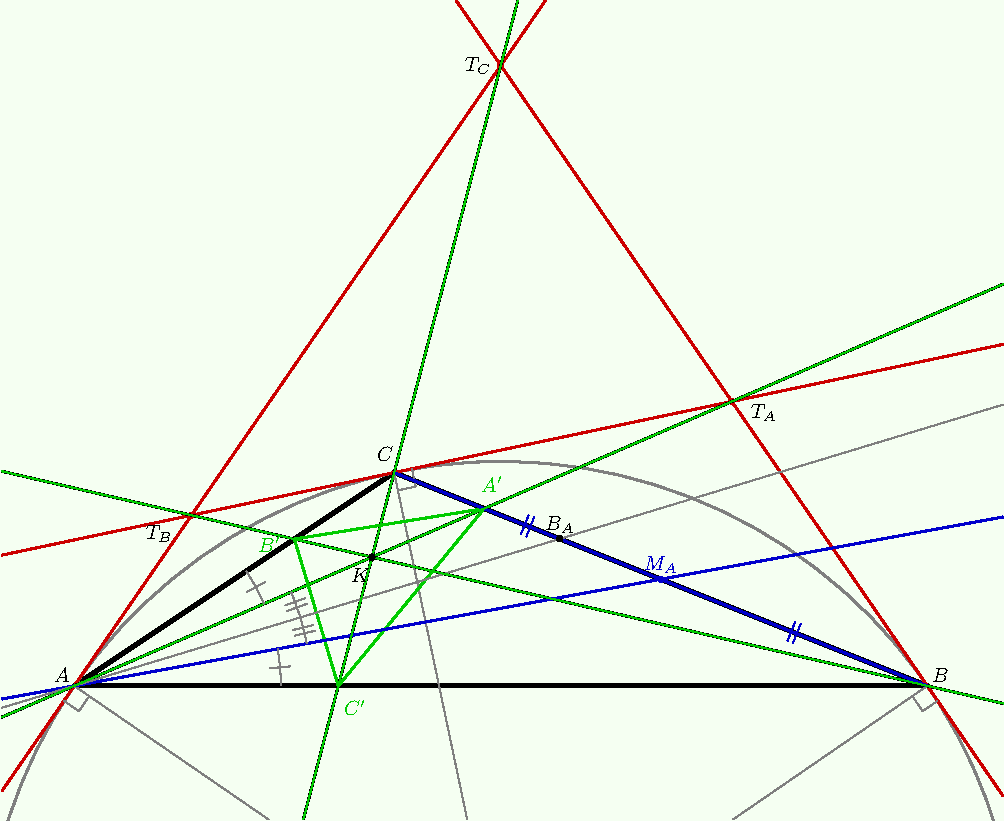
\includegraphics{include/symmedian_intro.pdf}
\end{center}
\hfill\hspace*{0mm}
\footnotetext[1]{%
  \begin{minipage}[t]{0.77\textwidth}
    Copyright \copyright{} 2007 Philippe Ivaldi.

    \begin{quotation}
      \noindent Permission is granted to copy, distribute and/or modify this document
      under the terms of the \emph{GNU} Lesser General Public License (see the
      file LICENSE in \href{http://git.piprime.fr/?p=asymptote/geometry-documentation.git;a=summary}{the top-level source directory}).
    \end{quotation}
  \end{minipage}}

\renewcommand{\thefootnote}{\arabic{footnote}}
\newpage

\begin{abstract}
  \noindent%
  This document deals with the use of \geo extension which
  makes the production of plane Euclidean geometry figures easier. \Geo
  extension defines some new types and routines for the
  \href{http://asymptote.sourceforge.net/}{\textsc{Asymptote}} software.\\
  First we will give the list with a brief description of the new
  types. Secondly we will study each of them and give details on the
  associated routines and operators.
  \begin{center}\bfseries
    Acknowledgements
  \end{center}
  I would like to thank
  \begin{itemize}
  \item Olivier \textsc{Guib�} for numerous discussions on some
    computer algebra questions, his encouragements and his always
    attentive listening;
  \item John \textsc{Bowman} and Andy \textsc{Hammerlindl} without
    \asymptote does not exist;
  \item \href{http://forum.mathematex.net/membre3.html}{MB} which has
    followed the development of this extension and has allowed to
    correct, improve and add some features.
  \end{itemize}
\end{abstract}
\newpage

\tableofcontents
\newpage

\hyperdef{section}{intro}{\section{Introduction}}%
%\section{Introduction}
\subsection{Objects types list}
\Geo defines many objects which are commonly used in plane Euclidean geometry;
as Asymptote provides the types \code{real} and \code{path} to handle real number and
path, \geo includes many structures and functions for geometry objects.
In the sequel it is important to distinguish an object and his type.
For instance  "Bivariate Quadratic Equation" is an object of type \code{bqe}
and possesses a named object \param{a} of type \code{real[]}; one can
accesses to it via the code  \code{an\_objet\_bqe.a}.\\
Here all the types provided by \geo:
\begin{description}
\item[\index{coordsys}coordsys] a cartesian coordinate system;
  this type is described in Section
  \href{#section.coordsys}{Coordinate system} and
  Section  \href{#section.point}{Points and vectors} explains his use;
\item[\index{point}point \textmd{and} \index{vector}vector] point and
  vector with respect to a cartesian coordinate system.\\
   The reading of Section  \href{#section.point}{Point and vectors}
   which deals with this types can be omitted if the reader does not
   want to use another coordinate system than the default one: in this case one
   can consider that the types \code{point} and \code{vector} are the
   same than the type \code{pair};
\item[\index{mass}mass] mass point with respect to a cartesian
  coordinate system   (cf. \href{#section.mass}{Mass points});
\item[\index{line}line \textmd{and} \index{segment}segment] the type
  \code{line} is devoted to  line, half-line or  segment.
  The type \code{segment}, for the definition of a segment, derives
  from the type \code{line} and is present to make easier the reading
  of the code.\\
  This types are described in Section
  \href{#section.line}{Lines, half-lines and segments};
\item[\index{conic}conic]
  conic of any type (cf. \href{#section.conic}{Conics}).\\
  For optimization's question\footnote{the method to compute the tangent to
    a circle is different in the case of an hyperbola} and code's
  reading the derived types
  \href{#subsection.circle}{circle},
  \href{#subsection.ellipse}{ellipse},
  \href{#subsection.parabola}{parabola},
  \href{#subsection.hyperbola}{hyperbola},
  \href{#subsubsection.bqe}{bqe} (for "Bivariate Quadratic
  Equation") are also defined.

  Therefore according to your aims, the more restrictive type of conic
  should be chosen; of course a particular conic can be converted into
  the general conic type as shown in the following example
    \begin{aVerbatim}
    ellipse a_circle=circle ((0,0), 3);
    ...
    conic a_conic=a_circle;
    ...
  \end{aVerbatim}
\item[\index{arc}arc] instance of an ellipse arc (cf. \href{#section.arc}{Arcs});
\item[\index{abscissa}abscissa] abscissa on a line (in the general sense) or on a conic
 (cf. \href{#section.abscissa}{Abscissa});
\item[\index{triangle}triangle] a triangle (cf. \href{#section.triangle}{Triangles}).\\
  The code \code{a\_triangle.object} allows to access to the objects
  which are connected to a triangle. Theses objects are of the types
  \begin{description}
  \item[\index{side}side] a triangle side (cf. \href{#subsection.side}{Sides});
  \item[\index{vertex }vertex] a triangle vertex
     (cf. \href{#subsection.vertex}{Vertexes}).
  \end{description}
\item[\index{trilinear}trilinear] trilinear coordinates with respect to
  a triangle (cf. \href{#subsection.trilinear}{Trilinear coordinates}).
\end{description}

\subsection{Internal running}
The computations on a object given by one of the types defined by \geo
are performed with respect to the nature of the object and not with
respect to his graphical representation which is finally a \code{path}
or a \code{pair}.

Indeed the following code which computes and draws the intersection
between two tangential circles is five times faster than an equivalent
routine which uses the type \code{path} in place of the type \code{circle}.
% \compiletrue%
\bvasy{circle_loop}
\subsection{Index and external examples}
An index and an examples gallery of all the routines, types and
operators defined in \geo allow a detailed view of this module:
\begin{itemize}
\item
  \href{http://piprim.tuxfamily.org/asymptote/geometry/modules/geometry.asy.index.sign.html}{index
    with respect to the name of function};
\item
  \href{http://piprim.tuxfamily.org/asymptote/geometry/modules/geometry.asy.index.type.html}{index
    with respect to the type of function};
\item
  \href{http://piprim.tuxfamily.org/asymptote/geometry/index.html}{examples gallery}.
\end{itemize}

\subsection{Casting }
The above cited objects can be processed by their own routines (the
ones defined by \geo) or by basic \asymptote routines thanks to the casting.
For example, a circle which is of type \code{circle} can be drawn
directly with the standard routine \code{draw} thanks to the automatic
casting \code{circle} into \code{path} while the code
\code{dot(a\_circle);} will return an error message because the
routine \code{dot}  {\bf exactly} needs  a type \code{path}; one must
force the casting with   the command \code{dot((path)a\_cercle);}.

\hyperdef{section}{coordsys}{\section{\index{Coordinate system|textbf}%
    \index{coordsys|textbf}Coordinate system}}

If you do not plan to use another coordinate system than the default one, this
section can be read later. In this case it is sufficient to know that
\geo uses the type \code{point} in place of the type \code{pair} and
that the types \code{vector} and \code{pair} are equivalent.

The following paragraphs deal with the basic routines on cartesian
coordinate systems, the real use of coordinate systems is detailed in Section \href{#section.point}{Points and vectors}.

\subsection{The type coordsys}
\Geo allows to define objects in any plane cartesian coordinate system ; such a
coordinate system is of the type \code{coordsys}. As shown below:
\begin{itemize}
\item  the default coordinate system is
  \index{coordsys!defaultcoordsys}\code{defaultcoordsys},
  which is the native one used by  \asymptote;
\item the current coordinate system is  \code{currentcoordsys} of which the
  default value is \code{defaultcoordsys}.
\end{itemize}
% \compiletrue%
\bvasy{defaultcoord}

\subsection{How to define a coordinate system}
\index{coordsys!cartesiansystem}\index{coordsys!currentcoordsys}
To define a coordinate system one can use the command
\code{cartesiansystem} or one can apply a transformation to some
coordinate system. For instance:
% \compiletrue%
\bvasy{cartesiancoord}

\subsection{Changing an object  pair on coordinate system}
\textbf{The examples of this section are given for information}, the
best method to define, modify, convert some coordinates into a coordinate system is to
use the type \code{point} (see \href{#section.point}{Points and vectors}).

Actually the two main ways to define or to convert some coordinates of the
type \code{pair} into a coordinate system are the operators:
\begin{itemize}
\item \index{coordsys!*}
  \begin{Vcolor}
    pair operator *(coordsys R, pair m)
  \end{Vcolor}
  convert the coordinates of \param{m} given in the coordinate
  system \param{R} into coordinates in the default coordinate system.
  Thus, in the following example, the point \param{M} has (0.5;0.5) for coordinates
  in \param{R} and (2;2) in \code{defaultcoordsys}:
  \bvasy{deftorel}
\item \index{coordsys!*}
  \begin{Vcolor}
    pair operator /( pair m, coordsys R)
  \end{Vcolor}
  convert the coordinates of \param{m} given in the default coordinate system
  into coordinates into the coordinate system \param{R}. Thus,
  in the following example, the points \param{M} and \param{P} have respectively
  the same coordinates in \param{R} and \param{Rp}:
  % \compiletrue%
  \bvasy{reltodef}
\end{itemize}

\subsection{Other routines}
\begin{itemize}
\item \index{coordsys!*}
  % \compiletrue%
  \begin{Vcolor}
    path operator *(coordsys R, path g)
  \end{Vcolor}
  a code of the type \code{coordsys*path} returns a new path which is
  a reconstruction of the path \param{g} given in the
  coordinate system \param{R}. It is a generalization of the
  \code{coordsys*pair} for paths.
\item \index{coordsys!*}
  % \compiletrue%
  \begin{Vcolor}
    coordsys operator *(transform t, coordsys R)
  \end{Vcolor}
  allow the code \code{transform*coordsys}. Observe that
  \code{shiftless(t)} is applied to \param{R.i} and \param{R.j}.
\end{itemize}

\hyperdef{section}{point}{\section{\index{point|textbf}Points and vectors}}
\subsection{The points}
\subsubsection{Basic principles}

While the type \code{pair} only allows to locate a point in the
default coordinate system, the type \code{point} allows to locate a point in any
cartesian coordinate system (see \href{#section.coordsys}{coordsys}); an object
of the type \code{point} refers to the coordinate system in which it is defined.

\index{point!casting}Thanks to the casting, a \code{point} is on the whole
 equivalent to a \code{pair} if one uses only the default coordinate system. Thus
 in the following example the \code{pair M} and the \code{point P}
 show the same point:
% \compiletrue%
\bvasy{point1}
\index{currentcoordsys}The following example shows the consequence of
a modification of the current coordinate system on the casting  \code{pair} in
\code{point} for the point \param{A} and how to define a point into a
specific coordinate system through to the routine \code{point point(coordsys R,  pair m)}
\index{point(coordsys,pair,real)} for the point \param{B}.
% \compiletrue%
\vasy{point2}
The routine \code{point locate(pair m);}\index{locate} also allows to
convert directly a \code{pair} into \code{point} without point's declaration:
% \compiletrue%
\bvasy{point3}
The example below shows how to convert a type \code{pair} into a type
\code{point} so that the result represents the same point and then how
to obtain his coordinates into  two distinct coordinate systems.
% \compiletrue%
\bvasy{point4}
The routine
\index{point!changecoordsys}\code{changecoordsys}
allows to change easily the coordinate system of a \code{point}:
% \compiletrue%
\vasy{point5}
\index{point!+}\index{point!-}\index{point!*}\index{point!/}

As for the type \code{pair} the operators \code{+}, \code{-},
\code{*}, \code{/} are available for the type \code{point}. Observe
that such an operation on two points defined into two
different coordinate systems gives a \code{point} defined into the default coordinate system
\code{defaultcoordsys}; a warning is given to the user about this
automatic conversion.

\index{coordsys!polar}\index{polar|see{coordsys polar}}
Locating a point with polar coordinate is possible via the code
\code{pair polar(real r, real angle)} of an object of the type
\code{coordsys} as shown in the following example:
% \compiletrue%
\bvasy{point6}

\subsubsection{Another routines}
Now that the basic routines concerning the type \code{point} are
defined, here we give another routines:
\begin{itemize}
\item \index{origin(coordsys)}
   %\compiletrue
  \begin{Vcolor}
    point origin(coordsys R=currentcoordsys)
  \end{Vcolor}
  Return the origin of the coordinate system \param{R} as a point.\\
  The constant \code{point origin}\index{origin} is the origin of the
  default coordinate system.
\item \index{point(coordsys,explicit point,real)}
  % \compiletrue
  \begin{Vcolor}
    point point(coordsys R, explicit point M, real m=M.m)
  \end{Vcolor}
  Return the point of mass \param{m} of which the relative coordinates
  to \param{R} are equal to the values of \param{M}.\\ Do not confuse
  this routine with  \code{changecoordsys}.

\item \index{coordinates(point)}
  % \compiletrue
  \begin{Vcolor}
    pair coordinates(point M)
  \end{Vcolor}
  Return the coordinates of \param{M} with respect to its coordinate system.

\item \index{samecoordsys(bool...point[])}
  % \compiletrue
  \begin{Vcolor}
    bool samecoordsys(bool warn=true ... point[] M)
  \end{Vcolor}
  Return \code{true} if and only if all the points are relative to the
  same coordinate system.\\
  If the value of \param{warm} is true and if the coordinate systems are
  different a warning is given.
\item \index{standardizecoordsys(coordsys,bool...M)}
  % \compiletrue
  \begin{Vcolor}
    point[] standardizecoordsys(coordsys R=currentcoordsys,
    bool warn=true ... point[] M)
  \end{Vcolor}
  Generalization of the routine \param{changecoordsys} to a array of
  points. Return, in a array form,  the points into the same
  coordinate system \param{R}. If the value of \param{warm} is true and if the
  coordinate systems of the points are different then a warning is given.
\item
  % \compiletrue
  \begin{Vcolor}
    pair[] operator cast(point[] P)
  \end{Vcolor}
  Casting of \code{point[]} into \code{pair[]}.
\item \index{locate(point)}
  % \compiletrue
  \begin{Vcolor}
    pair locate(point P)
  \end{Vcolor}
  Return the coordinates of \param{P} in the default coordinate system.
\item \index{*(transform,explicit point)}
  % \compiletrue
  \begin{Vcolor}
    point operator *(transform t, explicit point P)
  \end{Vcolor}
  Define \code{transform*point}.\\
  Remark that the transformations  \code{scale}, \code{xscale},
  \code{yscale} and \code{rotate} are defined with respect to the
  default coordinate system which is not wished in general when the current
  coordinate system has been modified.\\
  To make up for this inconvenient one can use the routines
  \code{scale(real,point)}, \code{xscale(real,point)},
  \code{yscale(real,point)},   \code{rotate(real,point)},
  \code{scaleO(real)},   \code{xscaleO(real)}, \code{yscaleO(real)} and
  \code{rotateO(real)} which are described in Section \href{section.transform1}{Transformations (Part 1)}.
\item \index{*(explicit point,explicit pair)}
  % \compiletrue
  \begin{Vcolor}
    point operator *(explicit point P1, explicit pair p2)
  \end{Vcolor}
  Define \code{point*pair}.\\
  We assume that the sense of \param{p2}  is a point of \param{p2}
  coordinates in the coordinate system where \param{P1} is defined (\code{point(coordinates(P1),p2)}).
\item \index{==(explicit point,explicit point)}
  % \compiletrue
  \begin{Vcolor}
    bool operator ==(explicit point M, explicit point P)
  \end{Vcolor}
  Define the test  \code{M == N} which returns  \code{true} if and
  only if  \code{MN < EPS}.
\item \index{!=(explicit point,explicit point)}
  % \compiletrue
  \begin{Vcolor}
    bool operator !=(explicit point M, explicit point N)
  \end{Vcolor}
  Define the test \code{M != N} which returns \code{true} if and only
  if \code{MN >= EPS}.
\item \index{abs(coordsys,pair)}
  % \compiletrue
  \begin{Vcolor}
    real abs(coordsys R, pair m)
  \end{Vcolor}
  Return the modulus $\vert$\param{m}$\vert$ with respect to the
  coordinate system \param{R}.
\item \index{abs(explicit point)}
  % \compiletrue
  \begin{Vcolor}
    real abs(explicit point M)
  \end{Vcolor}
  Return the modulus  $\vert\mparam{M}\vert$ with respect to its coordinate system.
\item \index{length(explicit point)}
  % \compiletrue
  \begin{Vcolor}
    real length(explicit point M)
  \end{Vcolor}
  Return the modulus  $\vert\mparam{M}\vert$  with respect to its coordinate system.
\item \index{conj(explicit point)}
  % \compiletrue
  \begin{Vcolor}
    point conj(explicit point M)
  \end{Vcolor}
  Return the conjugate of \param{M} with respect its coordinate
  system.
\item \index{degrees(explicit point,coordsys,bool)}
  % \compiletrue
  \begin{Vcolor}
    real degrees(explicit point M, coordsys,
    R=M.coordsys, bool warn=true)
  \end{Vcolor}
  Return the angle of \param{M} (in degrees) with respect to the  coordinate system \param{R}.
\item \index{angle(explicit point,coordsys,bool)}
  % \compiletrue
  \begin{Vcolor}
    real angle(explicit point M, coordsys,
    R=M.coordsys, bool warn=true)
  \end{Vcolor}
  Return the angle of \param{M} (in radians) with respect to the  coordinate system \param{R}.
\item \index{finite(explicit point)}
  % \compiletrue
  \begin{Vcolor}
    bool finite(explicit point p)
  \end{Vcolor}
  The same behavior than \code{finite(pair m)} in order to avoid
  computation with infinite coordinates.
\item \index{dot(point,point)}
  % \compiletrue
  \begin{Vcolor}
    real dot(point A, point B)
  \end{Vcolor}
  Return the dot product \param{A}{.}\param{B} with respect to the
  coordinate system of \param{A}.
\item \index{real dot(point,explicit pair)}
  % \compiletrue
  \begin{Vcolor}
    real dot(point A, explicit pair B)
  \end{Vcolor}
  Return the dot product  \param{A}{.}\param{B} where the coordinates
  of \param{A} are first converted into the default coordinate system.
  \code{dot(explicit pair,point)} is also defined.

\end{itemize}

\hyperdef{section}{vector}{\subsection{\index{vector|textbf}Vectors}}
\subsection{Basic principles}
In the following example the points \param{M} and \param{P} are
defined relatively to two different coordinate systems. The
point \param{Q}, namely the sum of \param{M} and \param{P}, is
obtained through the addition of the coordinates of \param{M}
and \param{P} \textbf{after their conversion into the default
  coordinate system}: thus  $\vec{\mbox{\param{OQ}}}=\vec{\mbox{\param{OM}}}+\vec{\mbox{\param{OP}}}$.

% \compiletrue
\bvasy{somme_point}
If we define the vector  $\vec{\mbox{\param{w}}}$ with \code{vector
  w=vector(R, P.coordinates);} (or in an easier way
\code{vector w=P;}) then we have
$\vec{\mbox{\param{w}}}=\vec{\mbox{\param{O}}_{1}\mbox{\param{P}}}$
and the code \code{point Q=M+w;} defines  \param{Q} such that
$\vec{\mbox{\param{OQ}}}=\vec{\mbox{\param{OM}}}+\vec{\mbox{\param{O}}_{1}\mbox{\param{P}}}$;
which is the expected result. Here an example

% \compiletrue
\bvasy{somme_point_vecteur}
An object \param{u} of the type \code{vector} has the same behavior
than an object of the type \code{point} but his conversion into
a \code{pair} or a \code{point} \param{M} relatively to the default
coordinate system is such that
$\vec{\mparam{u}}=\vec{\mparam{OM}}$. It is shown in the example below
which also uses the routine  \index{locate(vector)}\code{pair locate(vector v)}:
% \compiletrue
\bvasy{locate_vector}
The routines that are described for the type \code{point} are also
available for the type \code{point}. See below some simple examples:
% \compiletrue%
\bvasy{somme_vector}
% \compiletrue%
\vasy{somme_vector2}
\subsection{Vector/point casting}

With casting process an object \code{point} can be
converted into an object \code{vector} and mutually
an object \code{vector} can be converted into an object
\code{point}. If I may repeat myself it is important to
understand that the difference between \code{point} and \code{vector}
does not exist if you do not use another coordinate system than the
default one.


Observe in the following example the difference between  \code{dot(w)} and
\code{dot(point(w))}; in the second case the vector is converted into
a point, the one ``pointed out by the vector in the coordinate
system \param{R}'' while in the first case the
vector is converted into a \code{pair} as explained above.\\
Notice that it is possible to write  \code{point M=w;} in
place of \code{point M=point(w);}\index{point(explicit vector)}.
% \compiletrue%
\bvasy{locate_vector2}
The attentive reader will understand the following example:
% \compiletrue%
\bvasy{vector_point}
The counterpart of the routine  \code{point point(explicit vector)} is
\code{vector vector(point)}\index{vector vector(point)}:
% \compiletrue%
\bvasy{point_vector}

Finally  the reader must pay attention to the routines
\code{vector unit(point)}\index{unit(point)} and
\code{vector unit(vector)}\index{unit(vector)}
which always return an object  \code{vector}. Thus, in the following
example the behavior of \code{point P=unit(B-A);}  is not amazing
while the one of  \code{dot(unit(B-A))} can be dubious.
% \compiletrue%
\bvasy{unit_vector}
\subsection{Another routines}
\index{collinear(vector,vector)}As already mentioned all the routines
devoted to the type type \code{point} can also be used with the type
\code{vector}. Let us mention  the easily  understanding routine:
% \compiletrue%
\begin{Vcolor}
  bool collinear(vector u, vector v)
\end{Vcolor}

\hyperdef{section}{mass}{\section{\index{mass|textbf}Mass points}}
\hyperdef{subsection}{mass}{\subsection{Basic Principles}}

A \code{point} object possesses a mass which is attained with
\code{a\_point.m} and a routine allows to compute the center of a
points set.\\
``Perfect!''\\
No... not quite:
\begin{itemize}
\item if one defines the point  \param{M} with  \code{M=P1+P2;}, the
  mass of the point  \param{M} is the sum of the masses of  \param{P1}
  and \param{P2}, which is fine but if the point \param{M} is defined
  by  \code{M=P/2} the coordinates of \param{M} are well half the ones
  of \param{P} but the mass is unchanged. Thus to define a point with
  a half mass of a point we \textbf{should} write:

  % \compiletrue
  \begin{Vcolor}
    point P=point((1,1), 3);// point of mass 3

    point Q=P;
    Q.m=P.m/2;
  \end{Vcolor}
  which can become quickly painful;
\item to show the mass with an homogeneous way in all the figures at
  the time of using the routines \code{dot} and \code{label} can also
  be a painful task.
\end{itemize}
Mainly for this two reasons, \geo defines a new type, the type
\code{mass}\index{mass} which has at best an expected ``mass point''
behavior. For instance \code{mass M=object\_mass/2} defines the mass
point \param{M} with the same coordinates than \param{M} but a half
mass and the code \code{point M=object\_mass/2} has the same behavior
but the result is directly converted into \code{point}.

The routines \code{mass mass(explicit point)}\index{mass mass(explicit point)} and
\code{point point(explicit mass)}\index{point point(explicit mass)}
allow to overbalance easily between the two types  \code{mass} and
\code{point}; an elegant way to divide the mass of a \code{point}
object is then the following:

% \compiletrue%
\begin{Vcolor}
  point P=point((1,1), 3);// Point of mass 3

  point Q=mass(P)/2;// Division of the mass, the coordinates remain unchanged

\end{Vcolor}
The division of the coordinates of an object  of the type \code{mass}
is similarly:

\begin{Vcolor}
  mass P=mass((1,1), 3);// Mass weight equal to 3

  mass Q=point(P)/2;// Division of the coordinates, the weight remains unchanged

\end{Vcolor}
\subsection{Another  routines}
Thanks to the casting all the features of the type \code{point}
are available for the type \code{mass} with the already mentioned
nuances. Here the list of another routines in connections with the
mass points:
% \fvset{gobble=2}%
\begin{itemize}
\item \index{mass(coordsys,explicit pair,real)}
  % \compiletrue%
  \begin{Vcolor}
    mass mass(coordsys R, explicit pair p, real m)
  \end{Vcolor}
  Return an object of the type \code{mass} with a weight \param{m}
  from which the coordinates into \param{R} are \param{p}.
\item \index{mass(point,real)}
  % \compiletrue%
  \begin{Vcolor}
    mass mass(point M, real m)
  \end{Vcolor}
  Convert the point \param{M} into a mass of weight \param{m}.
\item \index{point(explicit mass)|textbf}
  % \compiletrue%
  \begin{Vcolor}
    point(explicit mass m)
  \end{Vcolor}
  Convert a mass of the type \code{mass} into a point of the type \code{point}.
\item \index{mass(explicit point)|textbf}
  % \compiletrue%
  \begin{Vcolor}
    mass mass(explicit point P)
  \end{Vcolor}
  Convert a point of the type \code{point} into a mass of the type \code{mass}.
\item \index{masscenter(...mass[])}
  % \compiletrue%
  \begin{Vcolor}
    mass masscenter(... mass[] M)
  \end{Vcolor}
  Compute the center of the masses array \param{M}.
  Thanks to the casting of \code{point[]} into \code{mass[]}, notice
  that this routine also works with a parameter of the type \code{point[]}.
\item \index{defaultmassformat}
  % \compiletrue%
  \begin{Vcolor}
    string defaultmassformat;
  \end{Vcolor}
  Default format used to construct the mass label.\\
  Its default value is
  \code{"\$$\backslash$left(\%L;\%.4g$\backslash$right)\$"}  in which
  \%L will be replaced by the label of the mass. The following
  example sheds a light on this routine:
  % \compiletrue%
  \bvasy{defaultmassformat}
  \vspace*{2mm}
\item \index{massformat(string,string,mass)}
  % \compiletrue%
  \begin{Vcolor}
    string massformat(string format=defaultmassformat,
    string s, mass M)
  \end{Vcolor}
  Return a string which is formated by the command \code{format}
  with \param{format} as parameter, in which \%L is replaced
  by \param{s} and the weight of \param{M}.

  % \compiletrue%
  \begin{Vcolor}
    import geometry;

    write(massformat(s="foo", mass((0,0),1000)));
    // Return $\left(foo;1000\right)$


    write(massformat("%L\_%e", "foo", mass((0,0),1000)));
    // Return foo\_1\!\times\!10^{3\phantom{+}}

  \end{Vcolor}
  \vspace*{2mm}
\item \index{void label(picture,Label,mass,align,string,pen,filltype)}
  % \compiletrue%
  \begin{Vcolor}
    void label(picture pic=currentpicture, Label L, mass M,
    align align=NoAlign, string format=defaultmassformat,
    pen p=nullpen, filltype filltype=NoFill)
  \end{Vcolor}
  Draw the label returned by \code{massformat(format,L,M)} at the coordinates of \param{M}.
\item \index{void label(picture,Label,mass,align,string,pen,filltype)}
  % \compiletrue%
  \begin{Vcolor}
    void dot(picture pic=currentpicture, Label L, mass M, align align=NoAlign,
    string format=defaultmassformat, pen p=currentpen)
  \end{Vcolor}
  Draw a dot into the point \param{M} and the label returned by  \code{massformat(format,L,M)}.
\end{itemize}

To conclude this section here are three examples using some of the
above described routines.
% \compiletrue%
\bvasy{mass_ex1}
% \compiletrue%
\bvasy{mass_ex2}
% \compiletrue%
The following example shows how one can construct all the partial
centers of \param{n} points, each center being connecting to the
points from which it is emerging.
\vasy{mass_ex3}

\hyperdef{section}{transform1}{\section{\index{transformation|textbf}Transformations
    (Part 1)}}
In addition to the native affine mappings \geo defines another plane
transformations. Some of them have a specific behavior with respect
the current coordinate system which is used. Thus, this section is
divided into two subsections. In the first one we study the mappings
which are independent of the current coordinate system. Secondly we
detail the coordinate system dependent transformations.
\subsection{Independent coordinate system mappings}
\begin{itemize}
\item \index{scale(real,point)}
  % \compiletrue
  \begin{Vcolor}
    transform scale(real k, point M)
  \end{Vcolor}
  Central similarity of center M and coefficient k.
  \bvasy{scale}
   \bvasy{scale2}
\item \index{projection(point,point)}
  % \compiletrue
  \begin{Vcolor}
    transform projection(point A, point B)
  \end{Vcolor}
  Orthogonal projection onto the line \param{(AB)}.
  \bvasy{projectionAB}
\item \index{projection(point,point,point,point,bool)}
  % \compiletrue
  \begin{Vcolor}
    transform projection(point A, point B, point C, point D, bool safe=false)
  \end{Vcolor}
  Return the projection along  \param{(CD)}  onto \param{(AB)}.\\
  If the value of \param{safe} is \code{true} and if the line  \param{(AB)}
  is parallel to the line \param{(CD)} then the identity is
  returned.\\
  If the value of \param{safe} is \code{false} and  if the line  \param{(AB)}
  is parallel to the line \param{(CD)} then the central similarity of
  center \param{O} and infinite coefficient is returned.
  \bvasy{projectionABCD}
\item \index{scale(real,point,point,point,point,bool)}
  % \compiletrue
  \begin{Vcolor}
    transform scale(real k, point A, point B, point C, point D, bool safe=false)
  \end{Vcolor}
  Return the affine transformation  of coefficient \param{k},
  of axis \param{(AB)} and of direction \param{(CD)}: if $M$ is point
  of the Euclidean plane the image $M'$ is defined by $P+k\vec{PM}$
  where $P$ is the projection along \param{(CD)} onto \param{(AB)} of
  the point $M$.\\
  If the value of \param{safe} is \code{true} and if the
  line \param{(AB)} is parallel to the line \param{(CD)}, the identity
  is returned.\\
  If the value of \param{safe} is \code{false} and if the
  line \param{(AB)} is parallel to the line \param{(CD)}, the central
  similarity of center \param{O} and infinite coefficient is returned.
  \bvasy{scaleABCD}
\end{itemize}
\subsection{Dependent coordinate system transformations}
\begin{itemize}
\item \index{xscale(real,point)}
  % \compiletrue
  \begin{Vcolor}
    transform xscale(real k, point M)
  \end{Vcolor}
  \hypertarget{xscale(real,point)}{Affine transformation} of
  coefficient \param{k}, of axis ``the line passing through \param{M} and
  parallel to \param{(Oy)}'' and of direction \param{(Ox)}.
  \bvasy{xscale1}
  The same example in any coordinate system:
  \index{xscale(real,point)}
  % \compiletrue
  \vasy{xscale2}
\item \index{yscale(real,point)}
  % \compiletrue
  \begin{Vcolor}
    transform yscale(real k, point M)
  \end{Vcolor}
  \hypertarget{yscale(real,point)}{Affine transformation} of
  coefficient \param{k}, of axis ``the line passing through \param{M} and
  parallel to \param{(Ox)}'' and of direction \param{(Oy)}.
  \bvasy{yscale1}
  The same example in any coordinate system:
  \index{yscale(real,point)}
  % \compiletrue
  \vasy{yscale2}
\item \index{scaleO(real)}
  % \compiletrue
  \begin{Vcolor}
    transform scaleO(real x)
  \end{Vcolor}
  Return the central similarity of coefficient  x and center ``the
  origin of the current coordinate system''. This transformation is
  equivalent to  \code{scale(x, origin())}.\\
  In the following example, one can see the difference between
  \code{scale(k)*P} and \code{scaleO(k)*P}.
  \bvasy{scaleO}
\item \index{xscaleO(real)}
  % \compiletrue
  \begin{Vcolor}
    transform xscaleO(real x)
  \end{Vcolor}
  Equivalent to \code{xscale(x, origin())} (see \href{#xscale(real,point)}{xscale(real,point)}).
\item \index{yscaleO(real)}
  % \compiletrue
  \begin{Vcolor}
    transform yscaleO(real x)
  \end{Vcolor}
  Equivalent to \code{yscale(x, origin())} (see \href{#yscale(real,point)}{yscale(real,point)}).
\item \index{rotateO(real)}
  % \compiletrue
  \begin{Vcolor}
    transform rotateO(real angle)
  \end{Vcolor}
  Equivalent to \code{rotate(angle, origin())}.
\end{itemize}

\hyperdef{section}{line}{\section{\index{line|textbf}Lines,
    half-lines and segments}}
\subsection{The type \texorpdfstring{``line''}{line}}
An object of type \code{line} is devoted  to describe  line,  half-line
or  segment depending on the properties value \code{bool
  extendA,extendB;} which is attained with the codes   \code{line.extendA} and
\code{line.extendB}.
The full description about the methods and properties of the type \code{line}
is accessible
\href{http://piprim.tuxfamily.org/asymptote/geometry/modules/geometry.asy.index.sign.html#struct\%20line}{here}.

\subsubsection{Lines defined by two points, basic routines}
\begin{itemize}
\item \index{line(point,bool,point,bool)}%
  % \compiletrue
  \begin{Vcolor}
    line line(point A, bool extendA=true, point B, bool extendB=true)
  \end{Vcolor}
  Define an object of type \code{line} passing through the two
  points  \param{A} and \param{B} and directed from \param{A}
  to \param{B}. If the value of \param{extendA} is \code{true} then
  the ``line'' goes on the side of \param{A}.

  An object of type \code{line} belongs to the coordinate system in
  which the two points \param{A} and \param{B} are defined. If it is
  not the case the two points are automatically redefined in the
  current coordinate system and a warning message is given.

\item \index{Ox()}\index{Oy()}\index{Ox}\index{Oy}%
  % \compiletrue
  \begin{Vcolor}
    line Ox(coordsys R=currentcoordsys)
  \end{Vcolor}
  Return the $x$-axis of the coordinate system \param{R}.\\
  The routine \code{line Oy(coordsys R=currentcoordsys)} is also
  defined.
  The constants \code{Ox} and \code{Oy} are the axis of the default
  coordinate system.
  \item \index{draw(picture,Label,line,bool,bool,align,pen,arrowbar,Label,marker)}%
  % \compiletrue
  \begin{Vcolor}
    void draw(picture pic=currentpicture, Label L="",
    line l, bool dirA=l.extendA, bool dirB=l.extendB,
    align align=NoAlign, pen p=currentpen,
    arrowbar arrow=None, Label legend="", marker marker=nomarker)
  \end{Vcolor}
  Draw into \param{pic} the ``line'' \param{l}  without changing the
  image size provide that the position of the Label is correct and
  that the variable \code{linemargin} is non negative.\\
    The boolean parameters \param{dirA} and \param{dirB} check the
  infinite part of the line to be drawn.\\
    Remark that the real variable \code{linemargin} allows to control
  the margin between the border of the image and the line drawing.
  The default value is 0 and  a negative value will change the size of
  the image.
    % \compiletrue%
  \bvasy{line_base}
\item \index{show(picture,line,pen)}%
  % \compiletrue%
  \begin{Vcolor}
    void show(picture pic=currentpicture, line l, pen p=red)
  \end{Vcolor}
  Draw into \param{pic} the points which are used to define the
  line \param{l} as well as the direction of the line and the
  orthogonal direction.
  \item \index{intersectionpoint(line,line)}%
  % \compiletrue%
  \begin{Vcolor}
    point intersectionpoint(line l1, line l2)
  \end{Vcolor}
  Return the intersection point between \param{l1} and \param{l2}.\\
    If the two lines do not intersect or if there is an infinite number
  of intersection points then this routine returns the point of
  coordinate \code{(infinity,infinity)}.
  Remark that if the two lines are defined into two different
  coordinate systems, the intersection point is defined into the
  default coordinate system and a warning message is given.\\
  The following example is an illustration of the famous Pascal
  theorem which claims that ``if a hexagon is inscribed in a conic,
  then the three points at which the pairs of opposite sides meet, lie
  on a straight line'' (here the conic is a circle).
    % \compiletrue
  \bvasy{th_pascal}
\item \index{intersectionpoints(line l, path g)}%
  % \compiletrue%
  \begin{Vcolor}
    point[] intersectionpoints(line l, path g)
  \end{Vcolor}
  Return an array of all the intersection points of the
  ``line'' \param{l} and the path \param{g}.
  \end{itemize}

\subsubsection{Lines defined by equations}
\begin{itemize}
\item \index{line(coordsys,real,real,real)}%
  % \compiletrue%
  \begin{Vcolor}
    line line(coordsys R=currentcoordsys, real a, real b, real c)
  \end{Vcolor}
  Return the line  described by the linear equation
  $\mparam{a}x+\mparam{b}y+\mparam{c}=0$ in the coordinate system \param{R}.
  \item \index{line(coordsys,real,real)}%
  % \compiletrue%
  \begin{Vcolor}
    line line(coordsys R=currentcoordsys, real slope, real origin)
  \end{Vcolor}
  Return the line of direction \param{slope} which the $y$-intersect
  is \param{origin} given in the coordinate system \param{R}.
  \end{itemize}
\subsubsection{Lines and parallelism}
\begin{itemize}
\item \index{parallel(point,line)}%
  % \compiletrue%
  \begin{Vcolor}
    line parallel(point M, line l)
  \end{Vcolor}
  Return the line passing through \param{M} which is parallel to \param{l}.
  \item \index{parallel(point,explicit vector)}%
  % \compiletrue%
  \begin{Vcolor}
    line parallel(point M, explicit vector dir)
  \end{Vcolor}
  Return the line of direction \param{dir} and passing through \param{M}.
  \item \index{parallel(point,explicit pair)}%
  % \compiletrue%
  \begin{Vcolor}
    line parallel(point M, explicit pair dir)
  \end{Vcolor}
  Return the line of direction \param{dir} given in the current
  coordinate system and passing through \param{M}.
  \item \index{parallel(line,line,bool)}%
  % \compiletrue%
  \begin{Vcolor}
    bool parallel(line l1, line l2, bool strictly=false)
  \end{Vcolor}
  Return \code{true} if \param{l1} is parallel to \param{l2} (strictly
  if the value of \param{strictly} is true).
  \end{itemize}
% \compiletrue%
\bvasy{parallel}
\subsubsection{Lines and angles}
\begin{itemize}
\item \index{line(real,point)}\index{line(point,real)}%
  % \compiletrue%
  \begin{Vcolor}
    line line(real a, point A=point(currentcoordsys,(0,0)))
  \end{Vcolor}
  Return the line passing through \param{A} and making an
  angle \param{a} with the $x$-axis of the coordinate system in
  which \param{A} is defined.\\
  The routine \code{line(point,real)} is also defined.
  \bvasy{line_angle1}
\item \index{bisector(line,line,real,bool)}%
  % \compiletrue%
  \begin{Vcolor}
    line bisector(line l1, line l2, real angle=0, bool sharp=true)
  \end{Vcolor}
  Return the image of the bisector of the angle between the two oriented
  lines \param{l1} and the \param{l2} by the rotation of center ``the
  intersection between the lines \param{l1} and \param{l2}'' and
  angle \param{angle}.\\
  If the value of \param{sharp} is \code{true}, this routine returns
  the internal bisector.\\
  Remark that the returned line inherits of the coordinate system
  in which the line \param{l1} is \hypertarget{bisectorline}{defined}.
  % \compiletrue%
  \bvasy{bisector_line}
\item \index{sector(int,int,line,line,real,bool)}%
  % \compiletrue%
  \begin{Vcolor}
    line sector(int n=2, int p=1, line l1, line l2, real angle=0, bool sharp=true)
  \end{Vcolor}
  Return the image of the $p$-th line which decompose the angle
  between the oriented lines \param{l1} and \param{l2} into \param{n}
  equal parts by the rotation of center  ``the
  intersection between the lines \param{l1} and \param{l2}'' and
  angle \param{angle}.\\
  If the value of \param{sharp} is \code{true}, this routine is
  performed on the acute angle.\\
  Remark that the returned line inherits of the coordinate system
  in which the line \param{l1} is defined.
  See below an example to decompose an angle into three equal measure parts.
  % \compiletrue%
  \vasy{sector_line}
\item \index{perpendicular(point,line)}%
  % \compiletrue%
  \begin{Vcolor}
    line perpendicular(point M, line l)
  \end{Vcolor}
  Return the line passing through \param{M} and perpendicular to the
  line \param{l}.
\item \index{line perpendicular(point,explicit vector)}%
  % \compiletrue%
  \begin{Vcolor}
    line perpendicular(point M, explicit vector normal)
  \end{Vcolor}
  Return the line passing through \param{M} and of orthogonal
  direction (or normal vector) \param{normal}.
\item \index{perpendicular(point,explicit pair)}%
  % \compiletrue%
  \begin{Vcolor}
    line perpendicular(point M, explicit pair normal)
  \end{Vcolor}
  Return the line passing through \param{M} and of orthogonal
  direction \param{normal} given in the current coordinate system \code{currentcoordsys}.
  % \compiletrue%
  \bvasy{perpendicular}
\item \index{angle(line,coordsys)}%
  % \compiletrue%
  \begin{Vcolor}
    real angle(line l, coordsys R=coordsys(l))
  \end{Vcolor}
  Return the radian measure of the angle, into  $(-\pi\,;\,\pi]$, with
  respect to the coordinate system \param{R} of the oriented
  line \param{l}, i.e. the angle between the oriented line and the $x$-axis.
\item \index{degrees(line,coordsys)}%
  % \compiletrue%
  \begin{Vcolor}
    real degrees(line l, coordsys R=coordsys(l))
  \end{Vcolor}
  Return the degree measure of the angle, into $[0\,;\,360)$, with
  respect to the  coordinate system \param{R} of the oriented
  line \param{l}, i.e.  the angle between the oriented line and the $x$-axis.
\item \index{sharpangle(line,line)}%
  % \compiletrue%
  \begin{Vcolor}
    real sharpangle(line l1, line l2)
  \end{Vcolor}
  Return the radian measure of the acute oriented angle, into
  $)-\frac{\pi}{2}\,;\,\frac{\pi}{2}]$, between \param{l1} and \param{l2}.
\item \index{sharpdegrees(line,line)}%
  % \compiletrue%
  \begin{Vcolor}
    real sharpdegrees(line l1, line l2)
  \end{Vcolor}
 Return the degree measure of the acute oriented angle, into
 $)-90\,;\,90]$, between \param{l1} and \param{l2}.
\item \index{angle(line,line)}%
  % \compiletrue%
  \begin{Vcolor}
    real angle(line l1, line l2)
  \end{Vcolor}
  Return the radian measure of the oriented angle, into
  $(-\pi\,;\,\pi]$, between the two oriented lines \param{l1} and \param{l2}.
\item \index{degrees(line,line)}%
  % \compiletrue%
  \begin{Vcolor}
    real degrees(line l1, line l2)
  \end{Vcolor}
  Return the degree measure of the oriented angle, into
  $(-180\,;\,180]$, between the two oriented lines \param{l1} and \param{l2}.
\end{itemize}
\subsubsection{Lines and operators}
\begin{itemize}
\item \index{*(transform,line)}%
  % \compiletrue%
  \begin{Vcolor}
    line operator *(transform t, line l)
  \end{Vcolor}
  Allow the code \code{transform*line}.
\item \index{/(line,real)}\index{*(real,line)}%
  % \compiletrue%
  \begin{Vcolor}
    line operator /(line l, real x)
  \end{Vcolor}
  Allow the code  \code{line/real}.\\
  Return the ``line'' passing through \param{l.A/x}
  and  \param{l.B/x}.\\
  The code \code{line operator *(real x, line l)} is also defined.
\item \index{*(point,line)}%
  % \compiletrue%
  \begin{Vcolor}
    line operator *(point M, line l)
  \end{Vcolor}
  Allow the code  \code{point*line}.\\
  Return the ``line'' passing through \code{unit(M)*l.A} and \code{unit(M)*l.B}.
\item \index{+(line,vector)}\index{-(line,vector)}%
  % \compiletrue%
  \begin{Vcolor}
    line operator +(line l, vector u)
  \end{Vcolor}
  Allow the code \code{line+vector}.\\
  Return the image of \param{l} by the translation of
  vector \param{u}.\\
  The code  \code{line operator -(line l, vector u)} is also defined.
\item \index{^^(line,line)}%
  % \compiletrue%
  \begin{Vcolor}
    line[] operator ^^(line l1, line l2)
  \end{Vcolor}
  Allow the code \code{line\circonflexe\circonflexe{}line}.\\
  Return the array \code{new line[] {l1,l2}}.
\item \index{==(line,line)}%
  % \compiletrue%
  \begin{Vcolor}
    bool operator ==(line l1, line l2)
  \end{Vcolor}
  Allow the test \code{line == line}.\\
  Return \code{true} if and only if the lines \param{l1} and \param{l2}
  are equal.
\item \index{!=(line,line)}%
  % \compiletrue%
  \begin{Vcolor}
    bool operator !=(line l1, line l2)
  \end{Vcolor}
  Allow the test \code{line != line}.\\
  Return \code{false} if and only if the lines \param{l1}
  and \param{l2} are equal.
\item \index{@(point,line)}%
  % \compiletrue%
  \begin{Vcolor}
    bool operator @(point m, line l)
  \end{Vcolor}
  Allow the code \code{point @ line}.\\
  Return \code{true} if and only if the point \param{M} belongs to the
  object \param{l}.
\end{itemize}
\subsubsection{Another routines}
In this section we describe routines which concern lines. Some of them
allow to get the \href{#section.abscissa}{abscissa} of a point
belonging to an object of type \code{line}.
\begin{itemize}
\item \index{draw(picture,Label[],line[],align,pen[],arrowbar,Label,marker)}%
  % \compiletrue%
  \begin{Vcolor}
    void draw(picture pic=currentpicture,Label[] L=new Label[], line[] l,
    align align=NoAlign, pen[] p=new pen[],
    arrowbar arrow=None,
    Label[] legend=new Label[], marker marker=nomarker)
  \end{Vcolor}
  Draw every line defined in the array \param{line[] l} with the
  pen corresponding to the array \param{pen[] p}.\\
  If \param{p} is not specified then the current pen is used.
\item \index{draw(picture,Label[],line[],align,pen,arrowbar,Label,marker)}%
  % \compiletrue%
  \begin{Vcolor}
    void draw(picture pic=currentpicture,Label[] L=new Label[], line[] l,
    align align=NoAlign, pen p,
    arrowbar arrow=None,
    Label[] legend=new Label[], marker marker=nomarker)
  \end{Vcolor}
  Draw every line defined in the array \param{line[] l} with the same
  pen \param{p}.\\
\item \index{distance(point,line)}\index{distance(line,point)}%
  % \compiletrue%
  \begin{Vcolor}
    real distance(point M, line l)
  \end{Vcolor}
  Return the distance from \param{M} to \param{l}.\\
  \code{real distance(line l,point M)} is also defined.
\item \index{sameside(point,point,line)}%
  % \compiletrue%
  \begin{Vcolor}
    bool sameside(point M, point P, line l)
  \end{Vcolor}
  Return \code{true} if and only if \param{M} and \param{P} are on the
  same side of \param{l}.
\item \index{sameside(point,line,line)}%
  % \compiletrue%
  \begin{Vcolor}
    point[] sameside(point M, line l1, line l2)
  \end{Vcolor}
  Return an array of two points: the first point is the projection of
  \param{M} onto \param{l1} along \param{l2} and the second one is the
  projection of \param{M} onto \param{l2} along \param{l1}.
\item \index{coordsys(line)}%
  % \compiletrue%
  \begin{Vcolor}
    coordsys coordsys(line l)
  \end{Vcolor}
  Return the coordinate system in which \param{l} is defined.
\item \index{changecoordsys(coordsys,line)}%
  % \compiletrue%
  \begin{Vcolor}
    line changecoordsys(coordsys R, line l)
  \end{Vcolor}
  Return the ``line'' described by \param{l} in the coordinate system \param{R}.
\item \index{reverse(line)}%
  % \compiletrue%
  \begin{Vcolor}
    line reverse(line l)
  \end{Vcolor}
  Return the ``line'' described by \param{l} with a contrary orientation.
\item \index{extend(line l)}%
  % \compiletrue%
  \begin{Vcolor}
    line extend(line l)
  \end{Vcolor}
  Return the line which contains \param{l} which can be an half line or a segment.
\item \index{complementary(explicit line)}%
  % \compiletrue%
  \begin{Vcolor}
    line complementary(explicit line l)
  \end{Vcolor}
  If \param{l} is an half line, it returns the complementary half line
  of \param {l}.
\item \index{concurrent(...line[])}%
  % \compiletrue%
  \begin{Vcolor}
    bool concurrent(... line[] l)
  \end{Vcolor}
  Return \code{true} if and only if the lines of the array
  \code{line[] l} are concurrent.
\item \index{perpendicular(line,line)}%
  % \compiletrue%
  \begin{Vcolor}
    bool perpendicular(line l1, line l2)
  \end{Vcolor}
  Return \code{true} if and only if the lines \param{l1}
  and \param{l2} are perpendicular.
\item \index{point(line l,real)}%
  % \compiletrue%
  \begin{Vcolor}
    point point(line l, real x)
  \end{Vcolor}
  Return the point between \param{l.A} and \param{l.B} as the code
  \code{point(l.A$--$l.B,x)} does.
\item \index{relpoint(line,real)}%
  % \compiletrue%
  \begin{Vcolor}
    point relpoint(line l, real x)
  \end{Vcolor}
  Return the point of relative abscissa \param{x} with respect to the
  oriented segment $[\mparam{AB}]$. In other words the
  codes \param{relpoint(l,x)} and \code{l.A+x*vector(l.B-l.A)} are
  equivalent.
  \bvasy{relpoint_line}
\item \index{curpoint(line,real)}%
  % \compiletrue%
  \begin{Vcolor}
    point curpoint(line l, real x)
  \end{Vcolor}
  Return the point of abscissa \param{x} with respect to the
  coordinate system  $(\mparam{l.A}\,;\,\vec{\mparam{l.u}})$.
  In other words the code \param{curpoint(l,x)} and
  \code{l.A+x*unit(l.B-l.A)} are equivalent.
  \bvasy{curpoint_line}
\end{itemize}


\subsubsection{Line and marker}
\begin{itemize}
\item \index{markangle(picture,Label,int,real,real,line,line,arrowbar,pen,margin,marker)}%
  % \compiletrue%
  \begin{Vcolor}
    void markangle(picture pic=currentpicture,
    Label L="", int n=1, real radius=0, real space=0,
    line l1, line l2,
    arrowbar arrow=None, pen p=currentpen,
    margin margin=NoMargin, marker marker=nomarker)
  \end{Vcolor}
  This routine marks  by  \param{n} circle arc(s) the oriented angle
  between the lines \param{l1} and \param{l2}. The arc(s) are drawn
  counterclockwise if \param{radius} is positive, clockwise otherwise.\\
  See \href{#bisectorline}{this figure} for an example.
\item \index{perpendicularmark(picture,line,line,real,pen,int,margin,filltype)}%
  % \compiletrue%
  \begin{Vcolor}
    void perpendicularmark(picture pic=currentpicture, line l1, line l2,
    real size=0, pen p=currentpen, int quarter=1,
    margin margin=NoMargin, filltype filltype=NoFill)
  \end{Vcolor}
  Mark a right angle to the intersection point of \param{l1}
  and \param{l2} in the \param{quarter}-th quarter of the plane
  counted in the counterclockwise, the first being the one delimited
  by the vectors \param{l1.u} and \param{l2.u}.
  \bvasy{perpendicularmark_line}
\end{itemize}

\subsection{The type \texorpdfstring{``segment''}{segment}}
As announced  in \href{#section.intro}{Introduction}, the type
\code{segment}, which deals with segment of line, derives from the
type \code{line}. With casting, almost all the routines
concerning the objects of type \code{line} are performed on a object
of type \code{segment} and conversely.

However observe that when a segment is drawn the value of the variable
\code{addpenline} is added to the used pen. The default value of this
variable is \param{squarecap} in order to have right ends. It follows
that the code \code{draw(a\_segment, dotted);} do not produce a
dotted segment.\\
There are three solutions to bypass this problem:
\begin{enumerate}
\item to write \code{draw(a\_segment,roundcap+dotted);} instead of
  \code{draw(a\_segment, dotted);}
\item to assign the variable \code{addpenline} the value \code{nullpen}
\item say to the author of \geo that you do not agree about the
  default value of \code{addpenline};
\end{enumerate}


At last, like we can switch the types \code{point} and \code{mass},
the objects of types \code{line} and \code{segment} can be converted
from one to another by writing for example
\code{segment s=an\_obj\_line;},\linebreak
\code{draw(segment(an\_obj\_line));} or
\code{draw(line(an\_obj\_segment));}.
The following example is an illustration
% \compiletrue
\bvasy{line_segment}
Apart from the routines defined for the \code{line} objects, we also
have some specific routines which deals with the \code{segment}
objects:
\begin{itemize}
\item \index{segment(point,point)}%
  % \compiletrue
  \begin{Vcolor}
    segment segment(point A, point B)
  \end{Vcolor}
  Return the line segment with the end points \param{A} and \param{B}.
\item \index{midpoint(segment)}%
  % \compiletrue
  \begin{Vcolor}
    point midpoint(segment s)
  \end{Vcolor}
  Return the midpoint of the segment \param{s}.
  % Renvoie le milieu du segment \param{s}.
\item \index{bisector(segment)}%
  % \compiletrue
  \begin{Vcolor}
    line bisector(segment s, real angle=0)
  \end{Vcolor}
  Return the image to the perpendicular bisector of \param{s} by the
  rotation of center ``the midpoint of \param{s}'' and angle \param{angle}.
\item \index{complementary(explicit segment)}%
  % \compiletrue
  \begin{Vcolor}
    line[] complementary(explicit segment s)
  \end{Vcolor}
  Return the two half-lines which contain the segment \param{s} and
  which have the end point \param{s.A} and \param{s.B} respectively.
\end{itemize}

\hyperdef{section}{transform2}{\section{\index{transformation|textbf}Affine
    Transformations (Part 2)}}
Some transformations which are defined from points in Section
\href{#section.transform1}{Affines transformations (Part 1)} can also
be defined from lines.
\begin{itemize}
\item \index{reflect(line)}
  % \compiletrue
  \begin{Vcolor}
    transform reflect(line l)
  \end{Vcolor}
  Return the reflection with respect to \param{l}.
  \bvasy{reflect}
\item \index{reflect(line,line,bool)}
  % \compiletrue
  \begin{Vcolor}
    transform reflect(line l1, line l2, bool safe=false)
  \end{Vcolor}
  Return the symmetry about \param{l1} in the direction \param{l2}.\\
  If the value \param{safe} is  \code{true} and if the lines \param{l1}
  and \param{l2} are parallel the routine returns the identity mapping.
  % \compiletrue
  \bvasy{reflect_dir}
\item \index{scale(real,line,line,bool)}
  % \compiletrue
  \begin{Vcolor}
    transform scale(real k, line l1, line l2, bool safe=false)
  \end{Vcolor}
  Return the affine transformation of coefficient $k$ of
  axis \param{l1} and direction \param{l2} (see the definition in
  Section 5.1, such an affine transformation is called
  ``affinity'').\\
  If the value of \param{safe} is \code{true} and if the
  lines \param{l1} and \param{l2} are parallel the routine returns the
  identity mapping.
  % \compiletrue
  \bvasy{affinite_line}
\item \index{projection(line)}
  % \compiletrue
  \begin{Vcolor}
    transform projection(line l)
  \end{Vcolor}
  Return the orthogonal projection onto the line \param{l}.
\item \index{projection(line)}
  % \compiletrue
  \begin{Vcolor}
    transform projection(line l1, line l2, bool safe=false)
  \end{Vcolor}
  Return the projection along \param{l2} onto \param{l1}.\\
  If the value of \param{safe} is \code{true} and if the
  lines \param{l1} and \param{l2} are parallel the routine returns the
  identity mapping.
\item \index{vprojection(line,bool)}
  % \compiletrue
  \begin{Vcolor}
    transform vprojection(line l, bool safe=false)
  \end{Vcolor}
  Return the projection onto \param{l} along the $y$-axis.\\
  It is equivalent to
  \code{projection(l,line(origin,point(defaultcoordsys,S)),safe)}.\\
  If the value of \param{safe} is \code{true} and if \param{l} is
  parallel to the $y$-axis the identity mapping is returned.
\item \index{hprojection(line,bool)}
  % \compiletrue
  \begin{Vcolor}
    transform hprojection(line l, bool safe=false)
  \end{Vcolor}
  Return the projection onto \param{l} along the $x$-axis.\\
  It is  equivalent to
  \code{projection(l,line(origin,point(defaultcoordsys,E)),safe)}.\\
  If the value of \param{safe} is \code{true} and if \param{l} is
  parallel to the $x$-axis the identity mapping is returned.
  % \compiletrue
  \bvasy{projection_line}
\end{itemize}

% \compiletrue
\hyperdef{section}{conic}{\section{\index{conique|mainidx}Conics}}
\subsection{The type ``conic''}
\subsubsection{Description}
\Geo defines the type \code{conic} to instantiate a conic section.
While it is quite possible to use an instance of this type, its
existence is rather intended for the internal workings of the
extension. We will prefer to use directly derived types \code{circle}, \code{ellipse},
\code{parabola} and \code{hyperbola} described later.

A look to its structure in order to define the
components:
% \compiletrue%
\begin{center}
  \begin{Vcolor}
    struct conic { real e, p, h; point F; line D; }
  \end{Vcolor}
\end{center}
\begin{itemize}
\item \param{e} is the eccentricity;
\item \param{F} is a focus and \param{D} the associated directrix;
\item \param{h} is the distance from \param{F} to \param{D};
\item \param{p} is the focal parameter ensuring the equality \param{p=he}.
\end{itemize}

The two main routines to define any conic are:

\begin{enumerate}
\item \index{conic conic(point,l,real)}
  % \compiletrue%
  \begin{Vcolor}
    conic conic(point F, line l, real e)
  \end{Vcolor}
  Return the conic specified by the focus \param{F}, which is associated to the
  directrix \param{l}, and eccentricity \param{e}; here is an example of use:
  % \compiletrue%
  \bvasy{conic_base}
\item \index{conic(point,point,point,point,point)}
  \begin{Vcolor}
    conic conic(point M1, point M2, point M3, point M4, point M5)
  \end{Vcolor}
  Return the non-degenerated conic passing through the
  points  \param{M1}, \param{M2}, \param{M3}, \param{M4}
  et \param{M5}.
  \vasy{conic_5_points}
\end{enumerate}
It should be noticed that it is also possible to define a conic
by its equation in a specified coordinate system, look at the section
\href{#subsection.bqe}{Conics equations}, and that other ways to
define a conic are implemented by routines referring to a specific
conic type which may be converted to type \code{conic}; look at
\href{#subsubsection.castingconic}{Conics and casting}.

\subsubsection{Basic routines}
The following routines may be used replacing an object of type conic
by one of types \code{circle}, \code{ellipse},
\code{parabola} or \code{hyperbola} except when the keyword
\code{explicit} precedes the type conic in the definition of the
routine.

It should be noted that, in addition to the routines described in this section,
exist routines returning an \href{#section.abscissa}{abscissa} of a point
onto an object of  type \code{conic}.
\begin{itemize}
\item \index{changecoordsys(coordsys,conic)}
  % \compiletrue
  \begin{Vcolor}
    conic changecoordsys(coordsys R, conic co)
  \end{Vcolor}
  Return the same conic as \param{co} relatively to the coordinate
  system \param{R}.
\item \index{coordsys(conic)}
  % \compiletrue
  \begin{Vcolor}
    coordsys coordsys(conic co)
  \end{Vcolor}
  Return the coordinate system in which the conic \param{co} is defined.
\item \index{canonicalcartesiansystem(explicit conic)}
  % \compiletrue
  \begin{Vcolor}
    coordsys canonicalcartesiansystem(explicit conic co)
  \end{Vcolor}
  \index{canonicalcartesiansystem(parabola)}
  \index{canonicalcartesiansystem(ellipse)}
  \index{canonicalcartesiansystem(hyperbola)}
  Return the canonical coordinate system of the conic \param{co}.\\
  The routines \code{canonicalcartesiansystem(ellipse)},
  \code{canonicalcartesiansystem(parabola)} and\linebreak
  \code{canonicalcartesiansystem(hyperbola)} are also available.\\
  The following example is an illustration in the case of an ellipse.
  \bvasy{canoniccoord}

\item \index{conicnodesnumber(conic,real,real)}
  % \compiletrue
  \begin{Vcolor}
    int conicnodesnumber(conic co, real angle1, real angle2, bool dir=CCW)
  \end{Vcolor}
  Return the nodes number used to convert the conic \param{co} to
  \code{path} between the angles \param{angle1} and \param{angle2}
  given in the direction of course \param{dir}.
\item \index{intersectionpoints(conic,conic)}
  % \compiletrue
  \begin{Vcolor}
    point[] intersectionpoints(conic co1, conic co2)
  \end{Vcolor}
  Return, in a array form, the intersection points of the two conics
  \param{co1} and \param{co2}.
  % \compiletrue
  \vasy{inter_conic}
\item \index{intersectionpoints(line,conic)}\index{intersectionpoints(conic,line)}
  % \compiletrue
  \begin{Vcolor}
    point[] intersectionpoints(line l, conic co)
  \end{Vcolor}
  Return, in a array form, the intersection points of the
  line \param{l} with the conic \param{co}.\\
  The routine \code{intersectionpoints(conic,line)} is also defined.
\item \index{intersectionpoints(conic,triangle,bool)}\index{intersectionpoints(triangle,conic,bool)}
  % \compiletrue
  \begin{Vcolor}
    point[] intersectionpoints(triangle t, conic co, bool extended=false)
  \end{Vcolor}
  Return, in an array form, the intersection points of the
  triangle \param{t} with the conic \param{co}. If \param{extended} is
  \code{true}, the sides of the triangle are regarded as extended
  lines; look at the section \href{#section.triangles}{Triangles}.\\
  The routine \code{intersectionpoints(conic,triangle,bool)} is also defined.
\end{itemize}

\subsubsection{Operators}
As with the previous routines, operators described here can be used by
replacing an object of type \code{conic} by one of the types
\code{circle}, \code{ellipse}, \code{parabola} or \code{hyperbola}.
\begin{itemize}
\item \index{@(point,conic)}
  % \compiletrue
  \begin{Vcolor}
    bool operator @(point M, conic co)
  \end{Vcolor}
  Allow the code \code{point @ conic}.\\
  Return \code{true} \ssi the point \param{M} belongs to the
  object \param{co}.
\item \index{*(transform,conic)}
  % \compiletrue
  \begin{Vcolor}
    conic operator *(transform t, conic co)
  \end{Vcolor}
  Allow the code \code{transform*conic}.
\item \index{+(conic,explicit point)}\index{-(conic,explicit point)}
  % \compiletrue
  \begin{Vcolor}
    conic operator +(conic co, explicit point M)
  \end{Vcolor}
  Allow the code \code{conic+point}.\\
  Return the image of the conic \param{co} by the translation of
  vector $\vec{O\mparam{M}}$.\\
  The routine \code{-(conic,explicit point)} is also defined.
\item \index{+(conic,explicit pair)}\index{-(conic,explicit pair)}
  % \compiletrue
  \begin{Vcolor}
    conic operator +(conic co, explicit pair m)
  \end{Vcolor}
  Allow the code \code{conic+pair}.\\
  Return the image of the conic \param{co} by the translation of
  vector $\vec{\mparam{Om}}$; $m$ represents the coordinates of a point
  defined relatively to the coordinate system in which the conic is
  defined.\\
  The routine \code{-(conic,explicit pair)} is also defined.
\item \index{+(conic,explicit vector)}\index{-(conic,explicit vector)}
  % \compiletrue
  \begin{Vcolor}
    conic operator +(conic co, explicit vector u)
  \end{Vcolor}
  Allow the code \code{conic+vector}.\\
  Return the image of the conic \param{co} by the translation of
  vector $\vec{\mparam{u}}$.\\
  The routine \code{-(conic,explicit vector)} is also defined.
\end{itemize}

\hyperdef{subsubsection}{bqe}{\subsubsection{\index{�quation!conique|mainidx}Conics equations}}
The type \code{bqe}, for \emph{Bivariate Quadratic Equation}, allows
to instantiate an object representing an conic equation in a given
coordinate system.  His structure follows:
\begin{center}
  \begin{Vcolor}
    struct bqe
    {
      real[] a;
      coordsys coordsys;
    }
  \end{Vcolor}
\end{center}
\noindent where:
\begin{itemize}
\item \param{a} is an arrow containing six coefficients of a conic equation
  given in the form \[\mparam{a[0]}x^2 + \mparam{a[1]}xy + \mparam{a[2]}y^2 + \mparam{a[3]}x + \mparam{a[4]}y + \mparam{a[5]}=0\]
\item \param{coordsys} is the coordinate system in which this
  equation is defined.
\end{itemize}
Here the list of routines regarding the objects of type \code{bqe}:
\begin{itemize}
\item \index{bqe(coordsys,real,real,real,real,real,real)}
  \begin{Vcolor}
    bqe bqe(coordsys R=currentcoordsys, real a, real b, real c, real d, real e, real f)
  \end{Vcolor}
  Return an object of type \code{bqe} representing the equation
  $\mparam{a}x^2 + \mparam{b}xy + \mparam{c}y^2 + \mparam{d}x + \mparam{e}y + \mparam{f}=0$
  relatively to the coordinate system \param{R}.
\item \index{changecoordsys(coordsys,bqe)}
  \begin{Vcolor}
    bqe changecoordsys(coordsys R, bqe bqe)
  \end{Vcolor}
  Return an object of type \code{bqe} relatively to the coordinate
  system \param{R} and representing the same conic than that
  represented by the parameter \param{bqe}. This routine allows to
  change the coordinate system of a bivariate quadratic equation.
\item \index{bqe(point,point,point,point,point)}
  \begin{Vcolor}
    bqe bqe(point M1, point M2, point M3, point M4, point M5)
  \end{Vcolor}
  Return an equation of the conic passing through the five
  points \param{M1}, \param{M2}, \param{M3}, \param{M4}
  and \param{M5}.\\
  If the points are defined relatively to the same coordinate system,
  the returned equation is relative to this coordinate system; else
  the equation is relative to the default coordinate system
  \code{defaultcoordsys}.
\item \index{conictype(bqe)}
  \begin{Vcolor}
    string conictype(bqe bqe)
  \end{Vcolor}
  Return the type of conic represented by \param{bqe}. The possible
  returned values are \code{"degenerated"}, \code{"ellipse"}, \code{"parabola"}
  and \code{"hyperbola"}.
\item \index{equation(explicit conic)}\index{equation(ellispe)}\index{equation(parabola)}\index{hyperbola}
  \begin{Vcolor}
    bqe equation(explicit conic co)
  \end{Vcolor}
  Return, in the form of object of type \code{bqe}, an equation of the
  conic \param{co}.\\
  The routines \code{equation(ellispe)}, \code{equation(parabola)} and
  \code{equation(hyperbola)} are also available.
\item \index{canonical(bqe)}
  \begin{Vcolor}
    bqe canonical(bqe bqe)
  \end{Vcolor}
  Return an equation of the conic represented by \param{bqe}
  relatively to the canonical coordinate system of the considered conic.
\item \index{conic(bqe)}
  \begin{Vcolor}
    conic conic(bqe bqe)
  \end{Vcolor}
  Return the conic represented by \param{bqe}
\end{itemize}

\hyperdef{subsubsection}{castingconic}{\subsubsection{\index{casting!conique|mainidx}Conics
    and casting}}
As already mentioned in the previous sections, the type conic can
instantiate an object representing any conic.
It is however possible, and often recommended, to convert an object
representing any conic in a specific type in order to use its own
properties and routines.

The specific types of conics are \code{circle}, which is a particular case
of the type \code{ellipse}, \code{parabola} and \code{hyperbola};
theses types are described in the sections below.

So in the example below the conical \param{co} is defined by a focus and the
corresponding directrix with an eccentricity less than 1. Since this
conic is an ellipse, one can assign to a variable of type
\code{ellipse} the variable \param{co} in order to extract its
dimensions.
\vasy{conic_ellipse}

From the point of view of the internal functioning of \geo some
routines that apply to an object of type \code{conic} call in fact
equivalent routines applying to a specific conic; this allows to
optimize some calculations. Conversely, routines for a specific
type of conic use underlying routines for any conics.

The specific types of conics are described below.

\hyperdef{subsection}{circle}{\subsection{\index{cercle|mainidx}\index{ellipse|mainidx}Circles}}
\subsubsection{basic routines}
Besides the routines for objects of type \code{conic}, here are some
other routines to define an object of type \code{circle}:
\begin{itemize}
\item \index{circle(explicit point,real)}%
  % \compiletrue%
  \begin{Vcolor}
    circle circle(explicit point C, real r)
  \end{Vcolor}
  Return the circle of radius \param{r} centered on \param{r}.\\
  Remark that the routine \code{circle circle(pair C, real r)} in no
  longer redefined since the \asymptote version 2{.}10�; one must use
  the casting of pair to point with the syntax \code{circle cle = circle((point)(1,2), 2)}
  whose center \param{(1,2)} represents the coordinates of a point in the
  current coordinate system \code{currentcoordsys}.

  The following example illustrates the difference between the code
  \code{circle((0,0),R);} which defines the blue circle in the
  current coordinate system and
  \code{circle(point(defaultcoordsys,(0,0)), R);}
  which defines the red circle in the default coordinate system;
  evidently, if the variable \param{currentcoordsys} is not modified,
  the two codes are equivalent.
  % \compiletrue%
  \bvasy{circlepointradius}
\item \index{circle(point A, point B)}%
  % \compiletrue%
  \begin{Vcolor}
    circle circle(point A, point B)
  \end{Vcolor}
  Return the circle of diameter \param{AB}.
\item \index{circle(point A, point B)}\index{circumcircle(point,point,point)}%
  % \compiletrue%
  \begin{Vcolor}
    circle circle(point A, point B, point C)
  \end{Vcolor}
  Return the circle passing through the distinct
  points \param{A}, \param{B} et \param{C}.\\
  An alias of this routine is \code{circle circumcircle(point A, point B, point C)}.
\item \index{incircle(point,point,point)}%
  % \compiletrue%
  \begin{Vcolor}
    circle incircle(point A, point B, point C)
  \end{Vcolor}
  Return the inscribed circle of the triangle ABC.
\item \index{excircle(point,point,point)}%
  % \compiletrue%
  \begin{Vcolor}
    circle excircle(point A, point B, point C)
  \end{Vcolor}
  Return the excircle of the triangle ABC tangent to (AB).
\end{itemize}
\index{clipdraw(picture,Label,path,align,pen,arrowbar,arrowbar,real,real,Label,marker)}%
In the example below we can see the use of the routine \code{clipdraw}
which draw a path by restricting the size of the final picture.
% \compiletrue%
\bvasy{circles_point}
Specific routines to the geometry of the triangle will achieve the
same result in a more elegant way, see the section
\href{#section.triangle}{Triangles}.

\subsubsection{From the type "circle" to the type "path"}
The casting of an object of type \code{circle} to type \code{path}
is done according to the following rules:
\begin{itemize}
\item the path is cyclic counterclockwise;
\item the first node of the path, as returned by the routine
  \code{pair point(path g, real t)}
  with \param{t=0}, is the intersection point of the circle with the
  half-line through the center and parallel to axis of the coordinate
  system in which the circle is defined;
\item the number of points of the path depends of the radius circle; it
  is calculated by the routine\linebreak
  \index{circlenodesnumber(real)}\code{int circlenodesnumber(real r)}
  which depends itself of the variable
  \index{circlenodesnumberfactor}\code{circlenodesnumberfactor}.
\end{itemize}
% \compiletrue%
\bvasy{circle_dot}
\subsubsection{The operators}
Apart from operators applying to objects of type \code{conic}, here
the list of others operator defined for the objects of type \code{circle}.
\begin{itemize}
\item \index{*(real,explicit circle)}\index{/(explicit circle,real)}%
  % \compiletrue%
  \begin{Vcolor}
    circle operator *(real x, explicit circle c)
  \end{Vcolor}
  Allow the code \code{real*circle}.\\
  Return the circle with same center as \param{c} and with radius \param{x}
  time that of \param{c}.\\
  The operator \code{circle operator /(explicit circle c, real x)} is
  also defined.
\item \index{\circonflexe(point M, explicit circle c)}%
  % \compiletrue%
  \begin{Vcolor}
    real operator ^(point M, explicit circle c)
  \end{Vcolor}
  Allow the code \code{point\circonflexe{}circle}.\\
  Return the circle power of \param{M} with respect to \param{c}.
\item \index{@(point,explicit circle)}%
  % \compiletrue%
  \begin{Vcolor}
    bool operator @(point M, explicit circle c)
  \end{Vcolor}
  Allow the code \code{point @ circle}.\\
  Return \code{true} \ssi the point \param{M} is on the circumference of \param{c}.
\item \index{circle to ellipse}%
  % \compiletrue%
  \begin{Vcolor}
    ellipse operator cast(circle c)
  \end{Vcolor}
  Allow the casting from \code{circle} to \code{ellipse}.\\
  The casting from \code{ellipse} to \code{circle} is also defined.\\
  One will note that the operator \code{*(transform t, circle c)} does
  not exist; through the casting, this is the operator \code{ellipse
    operator *(transform t, ellipse el)} which is used while executing
  the code \code{transform*circle}.\\
  Thus the code \code{scale(2)*circle} return an object of type
  \code{ellipse} but it is possible to write
  \code{circle=scale(2)*circle} while the code
  \code{circle=xscale(2)*circle} generates an error.
\end{itemize}

\subsubsection{Other routines}
Apart routines applied to objects of type \code{conic}, here is the
list of specific routines for objects of type \code{circle}.
\begin{itemize}
\item \index{radicalcenter(circle,circle)}%
  % \compiletrue%
  \begin{Vcolor}
    point radicalcenter(circle c1, circle c2)
  \end{Vcolor}
  Return the foot of the radical line of the two circle \param{c1}
  and \param{c2}.\\
  The coordinate system in which is defined the returned point is
  that of \param{c1}.
\item \index{radicalcenter(circle,circle,circle)}%
  % \compiletrue%
  \begin{Vcolor}
    point radicalcenter(circle c1, circle c2, circle c3)
  \end{Vcolor}
  Return the radical center of the three circles \param{c1}, \param{c2}
  and \param{c3}.
\item \index{radicalline(circle,circle)}%
  % \compiletrue%
  \begin{Vcolor}
    line radicalline(circle c1, circle c2)
  \end{Vcolor}
  Return the radical line of the two circles \param{c1}
  and \param{c2}.
\item \index{tangents(circle c, point M)}%
  % \compiletrue%
  \begin{Vcolor}
    line[] tangents(circle c, point M)
  \end{Vcolor}
  Return the eventual tangents to \param{c} passing through \param{M}.
  % \compiletrue
  \bvasy{tangentes_point_cercle}
\item \index{tangent(circle,abscissa)}
  % \compiletrue
  \begin{Vcolor}
    line tangent(circle c, abscissa x)
  \end{Vcolor}
  Return the tangent to \param{c} at the point whose the
  \href{#section.abscissa}{abscissa} is \param{x} on \param{c}.
\item \index{point(explicit circle,real)}
  % \compiletrue
  \begin{Vcolor}
    point point(explicit circle c, real x)
  \end{Vcolor}
  Return the \code{point} of \param{c} marking the same point than the
  returned \code{pair} by th code \code{point((path)c,x)}.
\item \index{relpoint(explicit circle,real)}
  % \compiletrue
  \begin{Vcolor}
    point relpoint(explicit circle c, real x)
  \end{Vcolor}
  Return the point of \param{c} corresponding to \param{x} time ``the
  perimeter of \param{c}''.
  \bvasy{relpoint_circle}
\item \index{angpoint(explicit circle,real)}
  % \compiletrue
  \begin{Vcolor}
    point angpoint(explicit circle c, real x)
  \end{Vcolor}
  Return the point of \param{c} corresponding with the angle \param{x}
  degrees.
  \bvasy{angpoint_circle}
\item \index{curpoint(explicit circle,real)}
  % \compiletrue
  \begin{Vcolor}
    point curpoint(explicit circle c, real x)
  \end{Vcolor}
  Return the point of \param{c} whose the curvilinear abscissa is \param{x}.
  \bvasy{curpoint_circle}
\end{itemize}
Others routines are defined for the objects of type \code{circle},
they are accessible via some routines using the type \code{ellipse}.

To conclude this section note that it is possible to use an object
of type \code{circle} as an inversion\index{inversion}. See
the section \href{#section.inversion}{Inversions} for further details.

Here are some examples of uses of routines previously described:
\begin{itemize}
\item Construction of two circles through the points $A$, $B$ and tangent
  to a given line $d$.
  % \compiletrue
  \vasy{circle_2pt_tangent}
\item \hypertarget{exemple_inversion}{Two points} of the plane and
  their inverses are cocyclic,
  on the orthogonal circle of the inversion circle.
  % \compiletrue
  \bvasy{inversion_pre}
\item Given three circles $\mathscr{C}_{1}$,
  $\mathscr{C}_{2}$ and $\mathscr{C}_{3}$ such as $r_{3}<r_{1}$ and
  $r_{3}<r_{2}$, how construct circles simultaneously tangent to these
  circles?

  The principle of construction illustrated below is as follows:
  \begin{itemize}
  \item If $S_{1}$ et $S_{2}$ are the inversions with positive radius
    transforming $\mathscr{C}_{2}$ to $\mathscr{C}_{3}$ and $\mathscr{C}_{1}$ to
    $\mathscr{C}_{3}$ respectively;
  \item considering a point $M$ on the cercle $\mathscr{C}_{3}$ and
    if $M_{1}$ and $M_{2}$ they images about $S_{1}$ et $S_{2}$ respectively;
  \item if $\mathscr{C}$ is the circle passing through $M$, $M_{1}$ and $M_{2}$;
  \item the radical line $(d)$ of circles $\mathscr{C}_{3}$ and
    $\mathscr{C}$ cuts the line passing through the inversions center
    $(S_{1}S_{2})$ in $H$; if $\mathscr{C'}$ is the cercle of diameter
    $\left[HO_{3}\right]$ where $O_{3}$ is the center of $\mathscr{C}_{3}$;
  \end{itemize}
  then:
  \begin{itemize}
  \item the circle $\mathscr{C'}$ cuts $\mathscr{C}_{3}$ in two points
    $T_{0}$ et $T_{1}$;
  \item the circle passing through $T_{0}$ and through the images $T'_{0}$ and
    $T''_{0}$ of $T_{0}$ about $S_{1}$ et $S_{2}$ respectively is one solution;
  \item the circle passing through $T_{1}$ and through the images $T'_{1}$ and
    $T''_{1}$ of $T_{1}$ about $S_{1}$ et $S_{2}$ respectively is an other solution;
  \end{itemize}
  % \compiletrue%
\vasy{apollonius}
\item Taking the four possible combinations for the inversions
  $S_{1}$ et $S_{2}$, we get the eight circles tangents to three
  given circles likewise:
  % \compiletrue%
\vasy{all_apollonius}
\end{itemize}

\hyperdef{subsection}{ellipse}{\subsection{\index{ellipse|mainidx}\index{ellipse|mainidx}Ellipses}}
The type \code{ellipse} does not surprise, it allows to
instantiate an object representing an ellipse.
As the type \code{circle} is a particular case of the type
\code{ellipse} it is possible to instantiate a circle as an ellipse zero eccentricity
and, reciprocally, to instantiate an zero eccentricity ellipse as a
circle.
Finally, as there is a one-to-one correspondence between objects of
type \code{ellipse} and those type \code{conic} with eccentricity
strictly less than $1$, objects of type \code{ellipse} inherit
routines and operators set for those type \code{conic}.

\subsubsection{Basic routines}
Here is a list of other routines to define a type \code{ellipse}.
\begin{itemize}
\item \index{ellipse(point,point,real)}
  \begin{Vcolor}
    ellipse ellipse(point F1, point F2, real a)
  \end{Vcolor}
  Return the ellipse foci \param{F1} and \param{F2} with semimajor axis \param{a}.
\item \index{ellipse(point,point,point)}
  \begin{Vcolor}
    ellipse ellipse(point F1, point F2, point M)
  \end{Vcolor}
  Return the ellipse foci \param{F1} and \param{F2} through \param{M}.
\item \index{ellipse(point,real,real,real)}
  \begin{Vcolor}
    ellipse ellipse(point C, real a, real b, real angle=0)
  \end{Vcolor}
  Return the ellipse centered at \param{C} with semimajor
  axis \param{a} in the direction given by \param{dir(angle)} and
  semiminor axis \param{b}.
  % \compiletrue
  \bvasy{ellipses_angle}
\end{itemize}
\subsubsection{From the type ``ellipse'' to the type ``path''}
The casting of an object of type \code{ellipse} to \code{path}
is done according to the following rules:
\begin{itemize}
\item the path is cyclic, counterclockwise oriented;
\item the first point, one returned by the routine \code{pair point(path
    g, real t)} with \param{t=0}, is the intersection point of the half
  focal line $[F_{1}F_{2})$ with the ellipse;
\item the nodes number of the path depends to the axis lengths of the
  ellipse; it is computed by the routine\linebreak
  \code{int ellipsenodesnumber(real a, real b)}\index{ellipsenodesnumber(real,real)}
  which itself depends on the variable
  \index{ellipsenodesnumberfactor}\code{ellipsenodesnumberfactor};
\item the nodes of the path are defined in polar coordinates with
  angles relatively to the center of the ellipse and evenly
  distributed throughout the interval $\left[0\,;\,360\right[$.
\end{itemize}
% \compiletrue%
\bvasy{ellipse_dot}

\subsubsection{Others routines}
Apart routines applied to objects of type \code{conic}, here is the
list of routines specific to objects of type \code{ellipse}.
\begin{itemize}
\item \index{focusToCenter(ellipse,real)}\index{centerToFocus(ellipse,real)}
  % \compiletrue
  \begin{Vcolor}
    real centerToFocus(ellipse el, real a)
  \end{Vcolor}
  Allow to convert an angle from the center of the ellipse to an angle
  form the first focus.\\
  The routine \code{real focusToCenter(ellipse,real)} is also defined.
\item \index{arclength(ellipse,real,real,bool,polarconicroutine)}
  % \compiletrue
  \begin{Vcolor}
    real arclength(ellipse el, real angle1, real angle2,
    bool direction=CCW,
    polarconicroutine polarconicroutine=currentpolarconicroutine)
  \end{Vcolor}
  Return the length of the ellipse arc defined by \param{el} from
  angle \param{angle1} to \param{angle2} (in degrees) in the
  direction \param{direction}.\\
  The possible values of \param{polarconicroutine}\index{polarconicroutine} are
  \code{arcfromfocus}\index{arcfromfocus}, which is the default value of\linebreak
  \code{currentpolarconicroutine}, or
  \code{arcfromcenter}\index{arcfromcenter}; in the first case the
  angles are relative to the first focus, in the second case, they are
  given relatively to the center of the ellipse.
\item \index{tangents(ellipse,point)}
  % \compiletrue
  \begin{Vcolor}
    line[] tangents(ellipse el, point M)
  \end{Vcolor}
  Return the eventual tangents to \param{el} through \param{M}.
  % \compiletrue
  \bvasy{tangentes_point_ellipse}
\item \index{tangent(ellipse,abscissa)}
  % \compiletrue
  \begin{Vcolor}
    line tangent(ellipse el, abscissa x)
  \end{Vcolor}
  Return the tangent to \param{el} at the \param{x}
  \href{#section.abscissa}{abscissa} point of \param{el}.

  The following example illustrates the definition of ellipse as
  the image of a circle by a dilatation and a related property of
  its tangents.
  % \compiletrue
  \vasy{affinite_cercle_ellipse_tgtes}
\item \index{point(explicit ellipse,real)}
  % \compiletrue
  \begin{Vcolor}
    point point(explicit ellipse el, real x)
  \end{Vcolor}
  Return the point of \param{el} which marks the same point as the
  \code{pair} returned by the code \code{point((path)el,x)}.
\item \index{relpoint(explicit ellipse,real)}
  % \compiletrue
  \begin{Vcolor}
    point relpoint(explicit ellipse el, real x)
  \end{Vcolor}
  Return the point of \param{el} which corresponds to the fraction \param{x}
  of the perimeter of \param{el}.
  \bvasy{relpoint_ellipse}
\item \index{angpoint(explicit ellipse,real)}
  % \compiletrue
  \begin{Vcolor}
    point angpoint(explicit ellipse el, real x,
    polarconicroutine polarconicroutine=currentpolarconicroutine)
  \end{Vcolor}
  Return the point of \param{el} with angle \param{x} degrees
  from the center of the ellipse\linebreak
  if \param{polarconicroutine=fromCenter}, from the first focus if
  \param{polarconicroutine=fromFocus}.
  \vasy{angpoint_ellipse}
\item \index{curpoint(explicit ellipse,real)}
  % \compiletrue
  \begin{Vcolor}
    point curpoint(explicit ellipse c, real x)
  \end{Vcolor}
  Return the point of \param{c} whose the curvilinear abscissa is \param{x}.
  \bvasy{curpoint_ellipse}
\end{itemize}

\hyperdef{subsection}{parabola}{\subsection{\index{parabole|mainidx}Paraboles}}
This is the type \code{parabola} which allows to instantiate a
parabola.
As there is a one-to-one correspondence between objects of type
\code{parabola} and those of type \code{conic} with eccentricity equal
to $1$, objects of type \code{parabola} inherit routines and operators
set for those of type \code{conic}.

\subsubsection{Basic routines}
The routines available to define a parabola are:
\begin{itemize}
\item \index{parabola(point,line)}
  % \compiletrue
  \begin{Vcolor}
    parabola parabola(point F, line l)
  \end{Vcolor}
  Return the parabola with focus \param{F} and directrix \param{l}.
\item \index{parabola(point,point)}
  \begin{Vcolor}
    parabola parabola(point F, point vertex)
  \end{Vcolor}
  Return the parabola with focus \param{F} and vertex \param{vertex}.
\item \index{parabola(point,real,real)}
  \begin{Vcolor}
    parabola parabola(point F, real a, real angle)
  \end{Vcolor}
  Return the parabola with focus \param{F}, with latus
  rectum \param{a} (the chord through a focus parallel to the conic
  section directrix) and whose the axis make an angle \param{angle}
  with the abscissa axis in which the point \param{F} is defined.
\item \index{parabola(point,point,point,line)}
  \begin{Vcolor}
    parabola parabola(point M1, point M2, point M3, line l)
  \end{Vcolor}
  Return the parabola through the
  points \param{M1}, \param{M2}, \param{M3} and whose the directrix is
  parallel to the line \param{l}.
  % \compiletrue
  \bvasy{parabole_3_points}
\end{itemize}

\subsubsection{From type ``parabola'' to type ``path''}
The casting of an object \param{P} of type \code{parabola} to \code{path}
is done according to the following rules:
\begin{itemize}
\item the path is oriented counterclockwise;
\item the path is content, if possible:
  \begin{enumerate}
  \item in the current picture if the variables \param{P.bmin}
    and \param{P.bmax}, type \code{pair},  have not been altered;
  \item in the rectangle \code{box((P.bmin),box(P.bmax))} otherwise.
  \end{enumerate}
  So in the following example, when the first conversion to path,
  the picture size is symbolized dashed and the path can not contain in
  this rectangle. During the second conversion, changing
  variables \param{p.bmin} and \param{p.bmax} redefines the area of
  conversion which is plotted in red with a corresponding portion of
  parabola.
  % \compiletrue
  \bvasy{parabola_to_path}
\item the number of nodes in the path depends on angles, given from
  focus in degrees, of the ends of the path and is calculated through the routine
  \index{parabolanodesnumber(parabola,real,real)}\code{int parabolanodesnumber(parabola p, real angle1, real angle2)}\linebreak
  which itself depends on the variable \index{parabolanodesnumberfactor}\code{parabolanodesnumberfactor};
\item the node in the path are defined in polar coordinates with
  angles given from parabola focus and evenly distributed throughout
  the interval whose ends are returned by the routine
  \code{real[] bangles(picture pic=currentpicture, parabola p)}\index{bangles(picture,parabola)}.
  % \compiletrue
  \bvasy{dot_parabola}
\end{itemize}

\subsubsection{Others routines}
Apart routines applied to objects of type \code{conic}, here the list
of specific routines to objects of type \code{parabola}.
\begin{itemize}
\item \index{tangents(parabola,point)}
  % \compiletrue
  \begin{Vcolor}
    line[] tangents(parabola p, point M)
  \end{Vcolor}
  Return the eventual tangents to \param{p} through \param{M}.
  \bvasy{tangentes_parabola}
\item \index{tangent(parabola,abscissa)}
  % \compiletrue
  \begin{Vcolor}
    line tangent(parabola p, abscissa x)
  \end{Vcolor}
    Return the tangent to \param{p} at the \param{x}
  \href{#section.abscissa}{abscissa} point of \param{p}.
\item \index{point(explicit parabola,real)}
  % \compiletrue
  \begin{Vcolor}
    point point(explicit parabola p, real x)
  \end{Vcolor}
    Return the point of \param{p} which marks the same point as the
  \code{pair} returned by the code \code{point((path)p,x)}.
\item \index{relpoint(explicit parabola,real)}
  % \compiletrue
  \begin{Vcolor}
    point relpoint(explicit parabola p, real x)
  \end{Vcolor}
    Return the point of \param{p} which marks the same point as the
  \code{pair} returned by the code \code{relpoint((path)p,x)}.
\item \index{angpoint(explicit parabola,real)}
  % \compiletrue
  \begin{Vcolor}
    point angpoint(explicit parabola p, real x)
  \end{Vcolor}
  Return the point of \param{p} with angle \param{x} degrees.
\item \index{curpoint(explicit parabola,real)}
  % \compiletrue
  \begin{Vcolor}
    point curpoint(explicit parabola p, real x)
  \end{Vcolor}
  Return the point of \param{p} whose the curvilinear abscissa
  is \param{x}, the origin being the vertex of the parabola.
  \bvasy{curpoint_parabola}
\item It is possible to obtain an arc of parabola in the form of
  \code{path} through the routine \index{arcfromfocus(conic,real,real,int,bool)}
  % \compiletrue
  \begin{Vcolor}
    path arcfromfocus(conic co, real angle1, real angle2, int n=400, bool direction=CCW)
  \end{Vcolor}
  Although this routine is available for any kind of conic its use has
  really of interest for the parabolas and hyperbolas; ellipse arcs have a
  specific type described in section \href{#section.arc}{Arcs}.

  Here an example illustrating the use of routine
  \code{arcfromfocus} with a parabola.
  \vasy{arcfromfocus_parabola}
\end{itemize}

\hyperdef{subsection}{hyperbola}{\subsection{\index{conique|mainidx}Hyperboles}}
This is the type \code{hyperbola} which allows to instantiate an
hyperbola.
As there is a one-to-one correspondence between objects of type
\code{hyperbola} and those of type \code{conic} with eccentricity
strictly greater than $1$, objects of type \code{hyperbola} inherit routines and operators
set for those of type \code{conic}.
\subsubsection{Basic routines}
The routines available to define an hyperbola are:
\begin{itemize}
\item \index{hyperbola(point,point,real,bool)}
  % \compiletrue
  \begin{Vcolor}
    hyperbola hyperbola(point P1, point P2, real ae, bool byfoci=byfoci)
  \end{Vcolor}
  \begin{description}
  \item[If \param{byfoci=true}:] return the hyperbola with semi-major axis
    \param{ae} and with foci \param{P1} and \param{P2};
  \item[If \param{byfoci=false}:] return the hyperbola with
    eccentricity \param{ae} and with vertices \param{P1} and \param{P2};
  \end{description}
  For more legibility, the constants \code{byfoci}\index{byfoci}
  and \code{byvertices}\index{byvertices} are defined, Their values
  are \code{true} and \code{false} respectively.
  \bvasy{hyperbole_def_1}
\item \index{hyperbola(point,real,real,real)}
  % \compiletrue
  \begin{Vcolor}
    hyperbola hyperbola(point C, real a, real b, real angle=0)
  \end{Vcolor}
  Return the hyperbola with center \param{C}, with semi-major axis \param{a}
  along \code{C{-}{-}C+dir(angle)} and with semi-minor axis \param{b}.
\item \index{conj(hyperbola)}
  \begin{Vcolor}
    hyperbola conj(hyperbola h)
  \end{Vcolor}
  Return the conjugate hyperbola of \param{h}.
  % \compiletrue
  \bvasy{conj_hyperbole}
\end{itemize}

\subsubsection{From type ``hyperbola'' to type ``path''}
The casting of an object \param{H} of type \code{hyperbola} to \code{path}
is done according to the following rules:
\begin{itemize}
\item the path is the hyperbola branch with focus \param{H.F1}
  oriented in trigonometric direction;
\item the path is contained, if possible:
  \begin{enumerate}
  \item in the current picture if the variable \param{H.bmin}
    and \param{H.bmax}, type \code{pair}, have not been changed;
  \item in the box \code{box((H.bmin),box(H.bmax))} otherwise.
  \end{enumerate}
    So in the following example, when the first conversion to path,
  the picture size is symbolized dashed and the path can not contain in
  this rectangle. During the second conversion, changing
  variables \param{H.bmin} and \param{H.bmax} redefines the area of
  conversion which is plotted in red with a corresponding portion of
  hyperbola.
  % \compiletrue
  \bvasy{hyperbola_to_path}
\item the number of node in the path depends on angles, given from
  focus in degrees, of the ends of the path and is calculated through the routine
  \code{int hyperbolanodesnumber(hyperbola p, real angle1, real angle2)}\index{hyperbolanodesnumber(hyperbola,real,real)}\linebreak
  which itself depends on the variable
  \index{hyperbolanodesnumberfactor}\code{hyperbolanodesnumberfactor};
\item the nodes in the path are defined in polar coordinates with
  angles given from focus \param{H.F1} and evenly distributed throughout
  the interval whose ends are returned by the routine
  \linebreak\code{real[][] bangles(picture pic=currentpicture, hyperbola p)}%
  \index{bangles(picture,hyperbola)}.
  % \compiletrue
  \bvasy{dot_hyperbola}
\end{itemize}

\subsubsection{Others routines}
Apart routines applied to objects of type \code{conic}, here the list
of specific routines to objects of type \code{hyperbola}.
\begin{itemize}
\item \index{tangents(hyperbola,point)}
  \begin{Vcolor}
    line[] tangents(hyperbola h, point M)
  \end{Vcolor}
  Return the eventual tangents to \param{p} through \param{M}.
  % \compiletrue
  \bvasy{tangents_hyperbola}
\item \index{tangent(hyperbola,abscissa)}
  % \compiletrue
  \begin{Vcolor}
    line tangent(hyperbola h, abscissa x)
  \end{Vcolor}
    Return the tangent to \param{h} at the \param{x}
    \href{#section.abscissa}{abscissa} point of \param{el}.
  \bvasy{tangent_hyperbola}
\item \index{point(explicit hyperbola,real)}
  % \compiletrue
  \begin{Vcolor}
    point point(explicit hyperbola h, real x)
  \end{Vcolor}
    Return the point of \param{h} which marks the same point as the
  \code{pair} returned by the code \code{point((path)h,x)}.
\item \index{relpoint(explicit hyperbola,real)}
  % \compiletrue
  \begin{Vcolor}
    point relpoint(explicit hyperbola h, real x)
  \end{Vcolor}
  Return the point of \param{h} which marks the same point as the
  \code{pair} returned by the code \code{relpoint((path)h,x)}.
\item \index{angpoint(explicit hyperbola,real,polarconicroutine)}
  % \compiletrue
  \begin{Vcolor}
    point angpoint(explicit hyperbola h, real x,
    polarconicroutine polarconicroutine=currentpolarconicroutine)
  \end{Vcolor}
  Return the point of \param{p} with angle \param{x} degrees from the
  hyperbola center \linebreak
  if \param{polarconicroutine=fromCenter}, from the first focus if
  \param{polarconicroutine=fromFocus}. Two examples are given further.
\item It is possible to obtain an arc of hyperbola in the form of
  \code{path} through the following routines\index{arcfromfocus(conic,real,real,int,bool)}
  \begin{enumerate}
    % \compiletrue
  \item
    \begin{Vcolor}
      path arcfromfocus(conic co, real angle1, real angle2, int n=400, bool direction=CCW)
    \end{Vcolor}
    Although this routine is available for any kind of conic its use has
    really of interest to the parabolas and hyperbolas; ellipse arcs have a
    specific type described in section \href{#section.arc}{Arcs}.

    Here an example illustrating the use of routine
    \code{arcfromfocus} with an hyperbola.
    \vasy{arcfromfocus_hyperbola}
  \item \index{arcfromcenter(hyperbola,real,real,int,bool)}
    \begin{Vcolor}
      path arcfromcenter(hyperbola h, real angle1, real angle2,
      int n=hyperbolanodesnumber(h,angle1,angle2), bool direction=CCW)
    \end{Vcolor}
    Here an example illustrating the use of routine
    \code{arcfromcenter} with an hyperbola.
    % \compiletrue
    \vasy{arcfromcenter_hyperbola}
  \end{enumerate}
\end{itemize}

\hyperdef{section}{arc}{\section{\index{arc|mainidx}Arcs}}
The type \code{arc} allows to instantiate an oriented ellipse
arc. The main routine to define a such arc is described
below\index{arc(ellipse,real,real,polarconicroutine,bool)}.
% \compiletrue
\begin{Vcolor}
  arc arc(ellipse el, real angle1, real angle2,
  polarconicroutine polarconicroutine=polarconicroutine(el),
  bool direction=CCW)
\end{Vcolor}
Return an arc of the ellipse \param{el} from angles (in
degrees) \param{angle1} to \param{angle2} in the
direction \param{direction} and given relatively to the first focus
if \param{polarconicroutine=fromFocus}, relatively to the center of
the ellipse if \param{polarconicroutine=fromCenter}.

The routine \code{polarconicroutine polarconicroutine(conic co)}%
\index{polarconicroutine(conic)} used here to determinate the default
value of the parameter \param{polarconicroutine} returns in this case
\code{fromCenter} if \param{co} represents a circle,
\code{currentpolarconicroutine}, which is \code{fromFocus} by default,
if \param{co} represents an ellipse.

It is important to note that, when drawn arc, the value of the
variable \code{addpenarc}\index{addpenarc} is added to the used
pen. By default this variable is set to \param{squarecap}, in order to
have the ends straight, which makes the display of a dotted arc inefficient.\\
To circumvent this problem there are three solutions:
\begin{enumerate}
\item write \code{draw(a\_arc, roundcap+dotted);} instead of
  \code{draw(a\_arc, dotted);};
\item set the value of \code{addpenarc} to \code{nullpen}.
\item contact the author of \geo to inform him of your disagreement
  with the default of \code{addpenline};
\end{enumerate}

Here are a few examples illustrating the use of routine\linebreak
\code{arc(ellipse,real,real,polarconicroutine,bool)}
\begin{itemize}
\item The following example shows how to obtain an ellipse arc whose
  angles are given from his first focus, that is the default behavior.
  Note the use of the routine
  \hyperdef{}{markarc}{\code{markarc}}\index{markarc} which will be
  described further.
  % \compiletrue
  \bvasy{arc_1}
\item The following example shows the effects of the parameters
  \param{polarconicroutine} and \param{direction}. Note the use of the
  routine \code{degrees(arc)} which will be described further.
  % \compiletrue
  \bvasy{arc_2}
\item The example below shows the previous code permuting the angles
  $45^{\circ}$ and $210^{\circ}$.
  \bvasy{arc_3}
\end{itemize}

\subsection{From type ``arc'' to type ``path''}
The casting of an object \param{A} of type \code{arc} to \code{path}
is done according to the following rules:
\begin{itemize}
\item the path is oriented in the direction \param{A.direction};
\item the number of nodes is computed by the routine\linebreak\index{arcnodesnumber(explicit arc)}%
  \code{int arcnodesnumber(explicit arc a)} which itself depends on the variable
  \index{ellispenodesnumberfactor}\code{ellispenodesnumberfactor};
\item the nodes in the path are defined in polar coordinates with
  angles given from the first focus or from the ellipse center
  depending to the value of \param{A.polarconicroutine} and evenly distributed throughout
  an adequate interval.
\end{itemize}
% \compiletrue
\bvasy{dot_arc}

\subsection{The operators}
\begin{itemize}
\item \index{*(transform,explicit arc)}
  \begin{Vcolor}
    arc operator *(transform t, explicit arc a)
  \end{Vcolor}
  Allow the code \code{transfomr*arc} whose behaviour is without
  surprise. In the following example the colored arcs are images of
  the black arc about affine transformations.
  % \compiletrue
  \vasy{transform_arc}
  The same example with an arc circle:
  % \compiletrue
  \bvasy{transform_arc_circle}
\item \index{*(real,explicit arc)}\index{/(explicit arc,real)}
  \begin{Vcolor}
    arc operator *(real x, explicit arc a)
  \end{Vcolor}
  Allow the code \code{real*arc}.

  Return the arc \param{a} with the angles \param{a.angle1-(x-1)*degrees(a)/2}
  and \param{a.angle2+(x-1)*degrees(a)/2}. The operator
  \code{/(explicit arc,real)} is also defined.

  In the following example the yellow arc is obtained multiplying
  the black arc by $0.5$ and the blue arc is obtained dividing it by $3$.
  % \compiletrue
  \bvasy{arc_mult_div_1}
  The same thing with an ellipse arc defined from the center of the ellipse.
  % \compiletrue
  \bvasy{arc_mult_div_2}
  Finally, in the following example, the arc is defined from the
  first focus of the ellipse:
  % \compiletrue
  \bvasy{arc_mult_div_3}
\item \index{+(explicit arc,point)}\index{-(explicit arc,point)}%
  \index{+(explicit arc,vector)}\index{-(explicit arc,vector)}
  \begin{Vcolor}
    arc operator +(explicit arc a, point M)
  \end{Vcolor}
  Allow the code \code{arc+point} which is an alias for \code{shift(point)*arc}.\\
  The operators
  \code{-(explicit arc,point)}, \code{+(explicit arc,vector)} and
  \code{-(explicit arc,vector)} are also defined.
\item \index{operator @(point,arc)}
  \begin{Vcolor}
    bool operator @(point M, arc a)
  \end{Vcolor}
  Allow the code \code{point @ arc}.
  Return \code{true} \ssi the point \param{M} belongs to the arc \param{a}.
\item \index{*(inversion,segment)}
  \begin{Vcolor}
    arc operator *(inversion i, segment s)
  \end{Vcolor}
  Allow the code \code{inversion*segment}.
  Return the image of \param{s} about the
  l'\href{#section.inversions}{inversion} \param{i}; one can
  \href{#inversion_damier}{look at the illustration} of
  \code{inversion*segment} at the section \href{#section.inversion}{Inversions}.
\end{itemize}

\subsection{Others routines}
In addition to the routines described in this section added routines
to locate a point on an object of type \code{arc} are described
in the section \href{#section.abscissa}{Abscissas}.
\begin{itemize}
\item \index{complementary(arc)}
  \begin{Vcolor}
    arc complementary(arc a)
  \end{Vcolor}
  Return the complementary of the arc \param{a}.
  % \compiletrue
  \bvasy{complementary_arc}
\item \index{reverse(arc)}
  \begin{Vcolor}
    arc reverse(arc a)
  \end{Vcolor}
  Return the reversed arc of \param{a} as would the routine
  \code{reverse(path)} does.
\item \index{degrees(arc)}\index{angle(arc)}
  \begin{Vcolor}
    real degrees(arc a)
  \end{Vcolor}
  Return the angle of the oriented arc \param{a} in degrees in the
  interval $\left[-360\,;\,360\right]$.\\
  The routine \code{angle(arc)} is also defined for angle in radians.
\item \index{arclength(arc a)}
  \begin{Vcolor}
    real arclength(arc a)
  \end{Vcolor}
  Return the length of the arc \param{a}.
\item \index{arclength(arc a)}
  \begin{Vcolor}
    void markarc(picture pic=currentpicture,
    Label L="", int n=1, real radius=0, real space=0,
    arc a, pen sectorpen=currentpen, pen markpen=sectorpen,
    margin margin=NoMargin, arrowbar arrow=None, marker marker=nomarker)
  \end{Vcolor}
  Allow to mark the angle \param{a} with an arc circle.\\
  The parameter \param{sectorpen} is the pen used to mark the segments
  which links the center or the focus of the arc with its ends.\\
  The parameter \param{markpen} is the pen used to draw the arc circle
  which may itself be marked with the parameter \param{marker}.\\
  \href{#markarc}{Examples} of use have already been given.
\item \index{intersectionpoints(arc,arc)}
  \begin{Vcolor}
    point[] intersectionpoints(arc a1, arc a2)
  \end{Vcolor}
  Return, in a array form, the intersection points of two arcs.
  The intersection routines of an object \code{arc} with
  others objects defined by \geo are also defined; for example
  \code{intersectionpoints(conic co, arc a)}\index{intersectionpoints(conic,arc)},
  \code{intersectionpoints(arc a, conic co)}\index{intersectionpoints(arc,conic)},
  \code{intersectionpoints(line l, arc a)}\index{intersectionpoints(line,arc)} etc...
\item \index{arcsubtended(point,point,real)}
  % \compiletrue
  \begin{Vcolor}
    arc arcsubtended(point A, point B, real angle)
  \end{Vcolor}
  Return the subtended arc of the line segment $[\mparam{AB}]$ with an
  angle \param{angle}. Although the code \code{a\_arcsubtended.C}
  allows to recover the center of the subtended arc, it is possible
  to obtain it using the routine\linebreak
  \code{point arcsubtendedcenter(point A, point B, real angle)}
  \index{arcsubtendedcenter(point,point,real)}.
  \bvasy{arcsubtended}
  \bvasy{angle_inscrit}
\item \index{arccircle(point,point,real,bool)}
  % \compiletrue
  \begin{Vcolor}
    arc arccircle(point A, point B, real angle, bool direction=CCW)
  \end{Vcolor}
  Return the arc circle, centered in \param{A}, from \param{B} to the
  image of \param{B} under the rotation with center \param{A} and
  angle \param{angle} in the direction \param{direction}.
  \bvasy{ove}
\item \index{arccircle(point,point,point)}
  % \compiletrue
  \begin{Vcolor}
    arc arccircle(point A, point M, point B)
  \end{Vcolor}
  Return the arc circle $\stackrel{\frown}{\mparam{AB}}$ through \param{M}.
  \bvasy{circumarc_def}
\item \index{arc(ellipse,point,point,bool)}
  % \compiletrue
  \begin{Vcolor}
    arc arc(ellipse el, point M, point N, bool direction=CCW)
  \end{Vcolor}
  Return the arc of \param{el}, with direction \param{direction},
  with ends \param{M} and \param{N} which must belong \param{el}.\\
  \vasy{arc_inter_points}
\item \index{arc(ellipse,abscissa,abscissa,bool)}
  \begin{Vcolor}
    arc arc(ellipse el, explicit abscissa x1, explicit abscissa x2, bool direction=CCW)
  \end{Vcolor}
  This routine has the same behavior as the previous routine but the
  points are specified with \href{#section.abscissa}{abscissas}
  relatively to the ellipse.
\item \index{arc(explicit arc,point,point)}
  \begin{Vcolor}
    arc arc(explicit arc a, point M, point N)
  \end{Vcolor}
  Return the arc part \param{a} between \param{M} and \param{N}.
  % \compiletrue
  \vasy{subarc_point}
\item \index{arc(arc,abscissa,abscissa)}
  \begin{Vcolor}
    arc arc(arc el, explicit abscissa x1, explicit abscissa x2)
  \end{Vcolor}
  This routine has the same behavior as the previous routine but the
  points are specified with \href{#section.abscissa}{abscissas}
  relatively to the ellipse.
\item \index{inverse(real,point,segment)}
  \begin{Vcolor}
    arc inverse(real k, point A, segment s)
  \end{Vcolor}
  Return the image of \param{s} under the inversion with
  center \param{A} and radius \param{k}; \href{#inversion_damier}{look
    at the illustration} of \linebreak \code{inversion*segment} in the
  section \href{#section.inversion}{Inversions}.
\item \index{tangent(explicit arc,point)}
  \begin{Vcolor}
    line tangent(explicit arc a, point M)
  \end{Vcolor}
  Return the tangent to \param{a} at point \param{M} of \param{a}.
\item \index{tangent(explicit arc,abscissa)}
  \begin{Vcolor}
    line tangent(explicit arc a, abscissa x)
  \end{Vcolor}
  Return the tangent to \param{a} at the point of
  \href{#section.abscissa}{abscissa} \param{x} given relatively to \param{a}.
\end{itemize}

\hyperdef{section}{abscissa}{\section{\index{abscisse|mainidx}Abscissas}}
The type \code{abscissa} allows to instantiate an abscissa on an object
of type \code{line}, \code{segment}, \code{conic} and \code{arc}. The
structure of an object of type \code{abscissa} follows:
\begin{center}
  \begin{Vcolor}
    struct abscissa {
      real x; int system; polarconicroutine
      polarconicroutine;
      abscissa copy() {...}
    }
  \end{Vcolor}
\end{center}
\begin{description}
\item[\param{x}] is the value of the abscissa.
\item[\param{system}] represents the type of abscissa:
  \begin{description}
  \item[0] for an abscissa as fraction of the length of path;
  \item[1] for a curvilinear abscissa;
  \item[2] for an angular abscissa;
  \item[3] for an abscissa relative to the nodes of a path.
  \end{description}
  For better readability of the code, the following constants are
  predefined\index{relativesystem}\index{curvilinearsystem}\index{angularsystem}\index{nodesystem}:
  \begin{Vcolor}
    int relativesystem=0, curvilinearsystem=1, angularsystem=2, nodesystem=3;
  \end{Vcolor}
\item[\param{polarconicroutine}] allow to specify the reference
  center in case of angular abscissa; the possible values are
  \code{fromCenter} and \code{fromFocus};
\item[\param{abscissa copy()}] return a deep copy of the abscissa.
\end{description}
\subsection{Define an abscissa}
There are as many routines to define an abscissa than type of
abscissa. Once an abscissa defined, one can recover the point of an
object to this abscissa with the routine \code{point(object,abscissa)}.
\begin{itemize}
\item \index{relabscissa(real)}
  \begin{Vcolor}
    abscissa relabscissa(real x)
  \end{Vcolor}
  Return the abscissa \param{x} as fraction of length of a path.
  It should be noted that the code \code{point(object,relabscissa(x))} is
  equivalent to \code{relpoint(object,x)}.
  % \compiletrue
  \bvasy{relabscissa}
\item \index{curabscissa(real)}
  \begin{Vcolor}
    abscissa curabscissa(real x)
  \end{Vcolor}
  Return the curvilinear abscissa \param{x}.
  It should be noted that the code \code{point(object,curabscissa(x))} is
  equivalent to \code{curpoint(object,x)}.
  % \compiletrue
  \bvasy{curabscissa}
\item \index{angabscissa(real,polarconicroutine)}
  \begin{Vcolor}
    abscissa angabscissa(real x,
    polarconicroutine polarconicroutine=currentpolarconicroutine)
  \end{Vcolor}
  Return the angular abscissa \param{x}.
  It should be noted that the code \code{point(object,angabscissa(x))} is
  equivalent to \code{angpoint(object,x)}.
  % \compiletrue
  \bvasy{angabscissa}
\item \index{nodabscissa(real)}
  \begin{Vcolor}
    abscissa nodabscissa(real x)
  \end{Vcolor}
  Return the abscissa \param{x} relative to the nodes of a path.
  It should be noted that the code \code{point(object,nodabscissa(x))} is
  equivalent to \code{point(object,x)}.
\end{itemize}

\subsection{Obtain an abscissa of a point}
The routines for obtaining an abscissa of a point belongs to a given
object have the same name as those described in the previous section.
The following routines return respectively the relative abscissa, the
curvilinear abscissa, the angular abscissa and the ``nodal abscissa''
of the point \param{M} belongs the specified object.
\begin{description}
\item[Relative abscissa]\hspace*{0mm}
  \begin{itemize}
  \item \index{relabscissa(line,point)}
    \begin{Vcolor}
      abscissa relabscissa(line l, point M)
    \end{Vcolor}
  \item \index{relabscissa(ellipse,point)}
    \begin{Vcolor}
      abscissa relabscissa(ellipse el, point M)
    \end{Vcolor}
  \item \index{relabscissa(arc,point)}
    \begin{Vcolor}
      abscissa relabscissa(arc a, point M)
    \end{Vcolor}
  \end{itemize}
\item[Curvilinear abscissa]\hspace*{0mm}
  \begin{itemize}
  \item \index{curabscissa(line,point)}
    \begin{Vcolor}
      abscissa curabscissa(line l, point M)
    \end{Vcolor}
  \item \index{curabscissa(ellipse,point)}
    \begin{Vcolor}
      abscissa curabscissa(ellipse el, point M)
    \end{Vcolor}
  \item \index{curabscissa(parabola,point)}
    \begin{Vcolor}
      abscissa curabscissa(parabola p, point M)
    \end{Vcolor}
  \end{itemize}
\item [Angular abscissa]\hspace*{0mm}
  \begin{itemize}
  \item \index{angabscissa(circle,point)}
    \begin{Vcolor}
      abscissa angabscissa(circle c, point M)
    \end{Vcolor}
  \item \index{angabscissa(ellipse,point,polarconicroutine)}
    \begin{Vcolor}
      abscissa angabscissa(ellipse el, point M, polarconicroutine
      polarconicroutine=currentpolarconicroutine)
    \end{Vcolor}
  \item \index{angabscissa(hyperbola,point,polarconicroutine)}
    \begin{Vcolor}
      abscissa angabscissa(hyperbola h, point M, polarconicroutine
      polarconicroutine=currentpolarconicroutine)
    \end{Vcolor}
  \item \index{angabscissa(parabola,point)}
    \begin{Vcolor}
      abscissa angabscissa(parabola p, point M)
    \end{Vcolor}
  \end{itemize}
\item[``Nodal abscissa'']\hspace*{0mm}
  \begin{itemize}
  \item \index{nodabscissa(line,point)}
    \begin{Vcolor}
      abscissa nodabscissa(line l, point M)
    \end{Vcolor}
  \item \index{nodabscissa(ellipse,point)}
    \begin{Vcolor}
      abscissa nodabscissa(ellipse el, point M)
    \end{Vcolor}
  \item \index{nodabscissa(parabola,point)}
    \begin{Vcolor}
      abscissa nodabscissa(parabola p, point M)
    \end{Vcolor}
  \end{itemize}
\end{description}

\subsection{Operators}
\index{+(real x, explicit abscissa a)}
\begin{Vcolor}
  abscissa operator +(real x, explicit abscissa a)
\end{Vcolor}
Return the copy of \param{a} with abscissa \param{x+a.x}.

The following operators are also efined:\\
\code{operator +(explicit abscissa,real)}\index{+(explicit abscissa,real)}\\
\code{operator -(real,explicit abscissa)}\index{-(real,explicit abscissa)}\\
\code{operator -(explicit abscissa,real)}\index{-(explicit abscissa,real)}\\
\code{operator -(explicit abscissa a)}\index{operator -(explicit abscissa a)}\\
\code{operator *(real x, explicit abscissa a)}\index{operator *(real x, explicit abscissa a)}\\
\code{operator *(explicit abscissa a, real x)}\index{operator *(explicit abscissa a, real x)}\\
\code{operator /(real x, explicit abscissa a)}\index{/(real x, explicit abscissa a)}\\
\code{operator /(explicit abscissa a, real x)}\index{/(explicit abscissa a, real x)}.

\hyperdef{section}{triangle}{\section{\index{triangle|mainidx}Triangles}}
\hyperdef{subsection}{struct}{\subsection{Structure}}
The \code{triangle} structure is more complex than the previous ones
already developed in this document. Indeed it defines new types which
create instances of some objects which are inextricably linked to a
triangle. Moreover these objects possess the reference of the
associated triangle.
In other words, an object \param{TR} of type \code{triangle} contains
as a structure member the
object \param{VA} of type \code{vertex} which is attained via the
code \param{TR.VA} and the object \param{TR.VA} contains the object \param{t} of type
\code{triangle} which value is \param{TR}; it follows that the value
of \param{TR.VA.t} is \param{TR}.

Since an object of type \code{vertex} is a triangle vertex, it is a
straightforward task to write a routine that returns for instance the
internal bisector of the angle of a triangle: it is sufficient to give
an object of type \code{vertex} since this object contains the
reference of the triangle of which it is a vertex.

Here is a simplified version of the \code{triangle} structure; the
complete structure is detailed \href{http://piprim.tuxfamily.org/asymptote/geometry/modules/geometry.asy.index.sign.html#struct\%20triangle}{separately}.
\begin{center}
  \begin{Vcolor}
    struct triangle {
      restricted point A, B, C;

      struct vertex {
        int n;
        triangle t; }

      restricted vertex VA, VB, VC;

      struct side {
        int n;
        triangle t; }

      side AB, BC, CA, BA, AC, CB; }
  \end{Vcolor}
\end{center}
\begin{description}
\item[\param{A}, \param{B} and \param{C}] represent the points marking
  the triangle vertices;
\item[\param{struct vertex}] defines the \code{vertex} structure which
  allows to create the instance of an object which represents the
  vertex of a triangle. Since we need to manipulate this structure in
  a very few cases, it is useful to know his properties.

  The property \param{n} allows to associated a vertex to a point, of
  type \code{point}, marking this vertex:\\
  if $\mparam{n}=1$, the vertex is associated to the
  point \param{A};\\
  if $\mparam{n}=2$, the vertex is associated to the
  point \param{B};\\
  if $\mparam{n}=3$, the vertex is associated to the
  point \param{C};\\
  if $\mparam{n}=4$, the vertex is associated to the
  point \param{A};\\
  etc.
  The value of the property \param{t} is ``the object of type
  \code{triangle} to which the vertex belongs''.\\
  For more details on the use of this structure see
  \href{#subsection.vertex}{Triangles vertices}.
\item[\param{VA}, \param{VB} et \param{VC}] represent the vertices of
  the triangle in an abstract way as opposed to the objects
  \code{point} \param{A}, \param{B} and \param{C} that are the points
  which mark each vertex; see Section
  \href{#subsection.vertex}{Triangles vertices}.
\item[\param{struct side}] defines the \code{side} structure which
  allows to create the instance of an object which represents
  the side of a triangle. Since we need to manipulate this structure in
  a very few cases, it is useful to know his properties.

  The property \param{n} allows to associated the object of type
  \code{side} to a triangle's side;\\
  if $\mparam{n}=1$, the side represents \param{AB} oriented
  from \param{A} to \param{B};\\
  if $\mparam{n}=2$, the side represents \param{BC} oriented
  from \param{B} to \param{C};\\
  if $\mparam{n}=3$, the side represents \param{CA} oriented
  from \param{C} to \param{A};\\
  if $\mparam{n}=4$, the side represents \param{AB};\\
  etc.

  if \param{n} is negative the orientation is reversed.\\
  The value of the property \param{t} is ``the object of type
  \code{triangle} to which the side belongs''.\\
  Routines on \param{side} are described into Section
  \href{#subsection.vertex}{Triangles sides}.
\item[\param{AB}, \param{BC}, \param{CA}, \param{BA}, \param{AC} et \param{CB}]
  represent the sides of the triangle in a abstract way as opposed to
  the objects \code{line} \param{line(TR.AB)}, \param{line(TR.BC)}, \param{line(TR.CA)},
  etc, that are the lines marking the sides of the
  triangle \param{TR}; see Section
  \href{#subsection.vertex}{Triangles sides}.
\end{description}

\subsection{Defining and drawing a triangle}

This section is devoted to describe the basic routines to define and
to draw a triangle. Another routines will be given as of reading.
\begin{itemize}
\item \index{label(picture,Label,Label,Label,triangle,real,real,pen,filltype)}
  \begin{Vcolor}
    void label(picture pic=currentpicture, Label LA="$A$",
    Label LB="$B$", Label LC="$C$",
    triangle t,
    real alignAngle=0,
    real alignFactor=1,
    pen p=nullpen, filltype filltype=NoFill)
  \end{Vcolor}
  Draw the labels \param{LA}, \param{LB} and \param{LC} at the
  vertices of the triangle \param{t}. The position depends on the
  internal bisector of the corresponding vertex. The
  parameters \param{alignAngle} and \param{alignFactor} allow to
  modify the direction and the length of the alignment.
\item \index{show(picture,Label,Label,Label,Label,Label,Label,triangle,pen,filltype)}
  \begin{Vcolor}
    void show(picture pic=currentpicture,
    Label LA="$A$", Label LB="$B$", Label LC="$C$",
    Label La="$a$", Label Lb="$b$", Label Lc="$c$",
    triangle t, pen p=currentpen, filltype filltype=NoFill)
  \end{Vcolor}
  Draw the triangle \param{t} and place the labels at the vertices of
  the triangle and the lengths of the sides. When coding this routine is useful to
  locate the vertices  \param{t.A}, \param{t.B} and \param{t.C}.
\item \index{drawline(picture,triangle,pen)}
  \begin{Vcolor}
    void draw(picture pic=currentpicture, triangle t,
    pen p=currentpen, marker marker=nomarker)
  \end{Vcolor}
  Draw the triangle  \param{t}; sides are drawn as segments.
\item \index{drawline(picture,triangle,pen)}
  \begin{Vcolor}
    void drawline(picture pic=currentpicture, triangle t, pen p=currentpen)
  \end{Vcolor}
  Draw the triangle \param{t}; sides are drawn as lines.
\item \index{triangle(point,point,point)}
  \begin{Vcolor}
    triangle triangle(point A, point B, point C)
  \end{Vcolor}
  Return the triangle whose vertices are  \param{A}, \param{B} et \param{C}.
\item \index{triangleabc(real,real,real,real,point)}
  \begin{Vcolor}
    triangle triangleabc(real a, real b, real c, real angle=0, point A=(0,0))
  \end{Vcolor}
  Return the triangle \param{ABC} such that
  $\mparam{BC}=\mparam{a}$, $\mparam{AC}=\mparam{b}$,
  $\mparam{AB}=\mparam{c}$ and
  $\left(\vec{\imath}\,;\,\vec{\mparam{AB}}\right)=\mparam{angle}$.
  % \compiletrue
  \bvasy{triangleabc}
\item \index{triangleAbc(real,real,real,real,point)}
  \begin{Vcolor}
    triangle triangleAbc(real alpha, real b, real c, real angle=0, point A=(0,0))
  \end{Vcolor}
  Return the triangle \param{ABC} such that
  $\left(\vec{\mparam{AB}}\,;\,\vec{\mparam{AC}}\right)=\mparam{alpha}$, $\mparam{AC}=\mparam{b}$,
  $\mparam{AB}=\mparam{c}$ et $ \left(\vec{\imath}\,;\,\vec{\mparam{AC}}\right)=\mparam{angle}$.
  % \compiletrue
  \bvasy{triangleAbc}
\item \index{triangle(line,line,line)}
  \begin{Vcolor}
    triangle triangle(line l1, line l2, line l3)
  \end{Vcolor}
  Return the triangle whose sides are  \param{l1}, \param{l2}
  and \param{l3}.
\end{itemize}

\hyperdef{subsection}{vertex}{\subsection{\index{vertex!triangle|mainidx}Vertices
    triangles}}

Let \param{t} be an object of type \code{triangle}. Its
properties \param{t.VA}, \param{t.VB} and \param{t.VC} are of type
\code{vertex} and describe the vertices of the
triangle \param{t}. \Geo allows routines with a vertex of triangle as
parameter without specifying explicitly the triangle to which it refers.

As an example in the following code the routine
\hypertarget{bisectorvertex}{%
  \code{line bisector(vertex V, real angle=0)}}%
\index{bisector(vertex,real)} returns the image by the rotation of
center \param{V} and angle \param{angle} of the internal bisector
passing through \param{V}.
\bvasy{bisector_vertex}
Here we have some routines and basic operators on the objects of type \param{vertex}
\begin{itemize}
\item \index{cast(vertex V)}
  \begin{Vcolor}
    point operator cast(vertex V)
  \end{Vcolor}
  Allow the casting  of  \code{vertex} in  \code{point}.
\item \index{point(explicit vertex V)}
  \begin{Vcolor}
    point point(explicit vertex V)
  \end{Vcolor}
  Return the object of type \code{point} corresponding to the
  object \param{V} of type \code{vertex}. The code \code{point(V)} is
  equivalent to the code \code{(point)V} which forces the casting of
  \code{vertex} in \code{point}.
\item \index{dir(vertex)}
  \begin{Vcolor}
    vector dir(vertex V)
  \end{Vcolor}
  Return the unit vector on the internal bisector of the angle
  in \param{V} and oriented outwards the triangle to which \param{V}
  refers. This routine is especially useful to place the labels at the
  vertices of a triangle.
\end{itemize}
Another routines with object of type \code{vertex} as parameter are
described in the following section and together with
\href{#subsection.routines}{routines regarding triangles}.

\hyperdef{subsection}{side}{\subsection{\index{side!triangle|mainidx}Sides
    triangles}}
Let \param{t} be an object of type \code{triangle}. Its properties
\param{t.AB}, \param{t.BC}, \param{t.CA}, \param{t.BA}, \param{t.AC}
and \param{t.CB}, of type \code{side} represents the sides of the
triangle \param{t}. \Geo  allows routines with a side of triangle as
parameter without specifying explicitly the triangle to which it refers.

As an example in the following code the routine
\hypertarget{excircleside}{\code{circle excircle(side
    s)}}\index{excircle(side)} returns the excircle of the
triangle to which~\param{s} refers and tangent to \param{s}.
\bvasy{excircle_intro}
Here we have some routines and basic operators on the objects of type \param{side}:
\begin{itemize}
\item \index{cast(side side)}
  \begin{Vcolor}
    line operator cast(side side)
  \end{Vcolor}
  Allow the casting of \code{side} in \code{line}.
\item \index{line(explicit side side)}
  \begin{Vcolor}
    line line(explicit side side)
  \end{Vcolor}
  Return the object of type \code{line} corresponding to the
  object \param{side} of type \code{side}. The code \code{line(S)} is
  equivalent to \code{(line)S} which forces the casting of \code{side}
  to \code{line}.
\item \index{segment(explicit side side)}
  \begin{Vcolor}
    segment segment(explicit side side)
  \end{Vcolor}
  Return the object of type  \code{segment} corresponding to the
  object \param{side} of type \code{side}. The code \code{segment(S)} is
  equivalent to \code{(segment)S} which forces the casting of
  \code{side} in \code{segment}.
\item \index{opposite(vertex)}
  \begin{Vcolor}
    side opposite(vertex V)
  \end{Vcolor}
  Return the opposite side to \param{V} about the triangle to
  which \param{V} refers.
\item \index{opposite(side)}
  \begin{Vcolor}
    vertex opposite(side side)
  \end{Vcolor}
  Return the opposite vertex to \param{side} into the triangle to
  which \param{side} refers.
\end{itemize}
The another routines with object of type \code{side} as parameter are
described together with \href{#subsection.routines}{routines regarding triangles}

\subsection{Operators}
The single operator which can be applied to \code{triangle} is
\index{*(transform,triangle)}
\begin{Vcolor}
  triangle operator *(transform T, triangle t)
\end{Vcolor}
\noindent that allows the code  \code{transform*triangle}.

\hyperdef{subsection}{routines}{\subsection{Another routines}}
\begin{itemize}
\item \index{orthocentercenter(triangle)}
  \begin{Vcolor}
    point orthocentercenter(triangle t)
  \end{Vcolor}
  Return the orthocenter of the triangle \param{t}.
\item \index{foot(vertex)}\index{foot(side)}
  \begin{Vcolor}
    point foot(vertex V)
  \end{Vcolor}
  Return the foot of the altitude from \param{V}. The routine
  \code{point foot(side side)} is also available.
\item \index{altitude(vertex)}\index{altitude(side)}
  \begin{Vcolor}
    line altitude(vertex V)
  \end{Vcolor}
  Return the altitude from \param{V}. The routine   \code{line
    altitude(side side)}  is also available.
\item \index{orthic(triangle)}
  \begin{Vcolor}
    triangle orthic(triangle t)
  \end{Vcolor}
  Return the orthic triangle of \param{t}; its vertices are the feet
  of the altitudes of \param{t}.
  \bvasy{orthic}
\item \index{midpoint(side)}
  \begin{Vcolor}
    point midpoint(side side)
  \end{Vcolor}
  Return the midpoint of \param{side}.
\item \index{centroid(triangle)}
  \begin{Vcolor}
    point centroid(triangle t)
  \end{Vcolor}
  Return the centroid of the triangle \param{t}.
\item \index{median(vertex)}\index{median(side)}
  \begin{Vcolor}
    line median(vertex V)
  \end{Vcolor}
  Return the median from \param{V}. The routine \code{line
    median(side side)} is also available.
\item \index{medial(triangle)}
  \begin{Vcolor}
    triangle medial(triangle t)
  \end{Vcolor}
  Return the medial triangle of \param{t} (its vertices are the
  midpoints of \param{t}).
  % \compiletrue
  \bvasy{medial}
\item \index{anticomplementary(triangle)}
  \begin{Vcolor}
    triangle anticomplementary(triangle t)
  \end{Vcolor}
  Return the anticomplementary triangle of \param{t} (\param{t} is
  the median triangle of \code{anticomplementary(t)}).
\item \index{bisector(vertex,real)}
  \begin{Vcolor}
    line bisector(vertex V, real angle=0)
  \end{Vcolor}
  Return the image of the internal bisector through \param{V}
  under the rotation of center \param{V} and angle \param{angle}. \href{#bisectorvertex}{An
  example} has already been given.
\item \index{bisectorpoint(side side)}
  \begin{Vcolor}
    point bisectorpoint(side side)
  \end{Vcolor}
  Return the intersection point of \param{side} with the internal bisector of the
   opposite angle to \param{side}.
\item \index{bisector(side side)}
  \begin{Vcolor}
    line bisector(side side)
  \end{Vcolor}
  Return the perpendicular bisector of the segment corresponding to \param{side}.
\item \index{circumcenter(triangle)}
  \begin{Vcolor}
    point circumcenter(triangle t)
  \end{Vcolor}
  Return the circumcenter of the triangle \param{t}.
\item \index{circle(triangle)}\index{circumcircle(triangle)}
  \begin{Vcolor}
    circle circle(triangle t)
  \end{Vcolor}
  Return the circumcircle of the triangle \param{t}. The routine
  \code{circumcircle(triangle t)} is an alias.
\item \index{tangential(triangle)}
  \begin{Vcolor}
    triangle tangential(triangle t)
  \end{Vcolor}
  Return the tangential triangle of \param{t}, that is the triangle
  whose sides are tangent to the circumcircle of \param{t}.
  % \compiletrue
  \bvasy{tangential}
\item \index{incenter(triangle)}
  \begin{Vcolor}
    point incenter(triangle t)
  \end{Vcolor}
  Return the incenter of \param{t}, that is the center of the
  incircle of \param{t}.
\item \index{inradius(triangle)}
  \begin{Vcolor}
    real inradius(triangle t)
  \end{Vcolor}
  Return the radius of the incircle of \param{t} (also known as the inradius).
\item \index{incircle(triangle)}
  \begin{Vcolor}
    circle incircle(triangle t)
  \end{Vcolor}
  Return the incircle of \param{t}.
\item \index{intouch(triangle)}
  \begin{Vcolor}
    triangle intouch(triangle t)
  \end{Vcolor}
  Return the contact triangle or intouch triangle that is the
  triangle whose vertices are the three points where the incircle
  touches the triangle \param{t}.
\item \index{intouch(side)}
  \begin{Vcolor}
    point intouch(side side)
  \end{Vcolor}
  Return the contact point of the side \param{side} with the incircle to which \param{side}
  refers.
\item \index{gergonne(triangle t)}
  \begin{Vcolor}
    point gergonne(triangle t)
  \end{Vcolor}
  Return the {\sc Gergonne} point of the triangle \param{t}.
  \bvasy{intouch}
\item \index{excenter(side)}
  \begin{Vcolor}
    point excenter(side side)
  \end{Vcolor}
  Return the center of the excircle of the triangle to
  which \param{side} refers and tangent to \param{side}.
\item \index{exradius(side)}
  \begin{Vcolor}
    real exradius(side side)
  \end{Vcolor}
  Return the radius of the excircle of the triangle to
  which \param{side} refers and tangent to \param{side}.
\item \index{excircle(side)}
  \begin{Vcolor}
    circle excircle(side side)
  \end{Vcolor}
  Return the excircle of the triangle to
  which \param{side} refers and tangent to \param{side}.
\item \index{extouch(triangle)}
  \begin{Vcolor}
    triangle extouch(triangle t)
  \end{Vcolor}
  Return the extouch triangle of \param{t} that is the triangle
  whose vertices are the contact points of the three excircles
  to \param{t} with its sides.
\item \index{extouch(side)}
  \begin{Vcolor}
    point extouch(side side)
  \end{Vcolor}
  Return the contact point of the side \param{side} with the excircle
  given by  \code{excircle(side)}.
  % \compiletrue
  \bvasy{extouch}
\item \index{symmedian(triangle)}
  \begin{Vcolor}
    point symmedian(triangle t)
  \end{Vcolor}
  Return the symmedian point (also called the \textsc{Lemoine} point) of the
  triangle \param{t}.
\item \index{symmedian(side side)}
  \begin{Vcolor}
    point symmedian(side side)
  \end{Vcolor}
  Return the symmedian point of the side \param{side}.
\item \index{symmedian(vertex V)}
  \begin{Vcolor}
    line symmedian(vertex V)
  \end{Vcolor}
  Return the symmedian line of the triangle to which \param{V} refers
  and passing through \param{V}.
  % \compiletrue
  \vasy{symmedian}
\item \index{cevian(side,point)}
  \begin{Vcolor}
    point cevian(side side, point P)
  \end{Vcolor}
  Return the {\sc Cevian} point of \param{P} belonging to the side \param{side}.
\item \index{cevian(triangle,point)}
  \begin{Vcolor}
    triangle cevian(triangle t, point P)
  \end{Vcolor}
  Return the
  \href{http://mathworld.wolfram.com/CevianTriangle.html}{{\sc Cevian}
    triangle} of \param{P}.
\item \index{cevian(vertex,point)}
  \begin{Vcolor}
    line cevian(vertex V, point P)
  \end{Vcolor}
  Return the {\sc Cevian} line of \param{P} passing
  through \param{V} in the triangle to which \param{V} refers.

  The following example is an illustration of the property ``\emph{if the
    triangle  $A'B'C'$ is a \textsc{Cevian} triangle of the triangle $ABC$
    then the triangle  $A''B''C''$ whose vertices are the symmetric of
    $A'$, $B'$ et $C'$  about the respective midpoints is also
    a  \hypertarget{cevian_ex}{\textsc{Cevian}} triangle}''.
  % \compiletrue
  \vasy{cevian}
\item \index{isotomic(vertex,point)}
  \begin{Vcolor}
    line isotomic(vertex V, point M)
  \end{Vcolor}
  Return the
  \href{http://mathworld.wolfram.com/IsotomicLines.html}{isotomic
    line} through \param{V} and relative to \param{M} about the
  triangle which \param{V} refers.
\item \index{isotomicconjugate(triangle,point)}
  \begin{Vcolor}
    point isotomicconjugate(triangle t, point M)
  \end{Vcolor}
  Return the
  \href{http://mathworld.wolfram.com/IsotomicLines.html}{isotomic
    conjugate} of \param{M} relatively to \param{t}.
\item \index{isotomic(side,point)}
  \begin{Vcolor}
    point isotomic(side side, point M)
  \end{Vcolor}
  Return the intersection point of the
  \href{http://mathworld.wolfram.com/IsotomicLines.html}{isotomic
    line} of \param{M}, about the triangle
  which \param{side} refers, with the side \param{side}.
\item \index{isotomic(triangle,point)}
  \begin{Vcolor}
    triangle isotomic(triangle t, point M)
  \end{Vcolor}
  Return the triangle whose the vertices are the intersection points of
  the isotomic lines relative to \param{M} about \param{t} with the sides
  of \param{t}. So, in \href{#cevian_ex}{the previous picture}, the
  triangle $A''B''C''$ is the isotomic triangle relative to \param{P}.

  Below, the same figure obtained using routines \code{isotomic} gains
  in brevity.
  % \compiletrue
  \vasy{isotomic}
\item \index{isogonalconjugate(triangle,point)}
  \begin{Vcolor}
    point isogonalconjugate(triangle t, point M)
  \end{Vcolor}
  Return the
  \href{http://en.wikipedia.org/wiki/Isogonal_conjugate}{isogonal
    conjugate} of \param{M} about \param{t}.
\item \index{isogonal(side,point)}
  \begin{Vcolor}
    point isogonal(side side, point M)
  \end{Vcolor}
  Return the intersection point of the
  \href{http://mathworld.wolfram.com/IsogonalLine.html}{isogonal line}
  of \param{M}, according to the triangle which \param{side} refers, with the
  side \param{side}.
\item \index{isogonal(triangle,point)}
  \begin{Vcolor}
    triangle isogonal(triangle t, point M)
  \end{Vcolor}
  Return the triangle whose the vertices are the intersection points
  with the sides of \param{t} of the isogonal lines relative
  to \param{M} about \param{t}.\\
  The following example illustrates the property \emph{"the pedal triangles
  of two isogonal points $P$ and $Q$ are inscribed in the same circle
  centered at the midpoint of the segment line $[PQ]$."}
% \compiletrue
  \vasy{isogonaux}
\item \index{pedal(triangle,point)}
  \begin{Vcolor}
    triangle pedal(triangle t, point M)
  \end{Vcolor}
  Return the
  \href{http://mathworld.wolfram.com/PedalTriangle.html}{pedal triangle} of \param{M} about \param{t}.
\item \index{pedal(side side, point M)}
  \begin{Vcolor}
    line pedal(side side, point M)
  \end{Vcolor}
  Return the line through \param{M} and through the foot of the
  perpendicular from \param{M} to the side line  \param{side}.\\
  The following example shows a few lines of \textsc{Simson}; note
  the use of methods \code{t.side(int)} and \code{t.vertex(int)} that
  allows to obtain by theirs numbers the sides and the vertices of the triangle
  \param{t}.
  % \compiletrue
  \bvasy{simson}
  % \compiletrue
\item \index{antipedal(triangle,point)}
  \begin{Vcolor}
    triangle antipedal(triangle t, point M)
  \end{Vcolor}
  Return the triangle whose the pedal triangle of \param{M} is \param{t}.
  \bvasy{antipedal}
\end{itemize}
\hyperdef{subsection}{trilinear}{\subsection{\index{trilinear!coordinates|mainidx}%
    \index{trilinear toordinates!triangle|mainidx}Trilinear coordinates}}
The type \code{trilinear}, whose the structure is given further,
allows to instantiate an object representing the
\href{http://mathworld.wolfram.com/TrilinearCoordinates.html}{trilinear
  coordinates} \param{a:b:c} with respect to the triangle~\param{t}.
\begin{center}
  \begin{Vcolor}
    struct trilinear
    {
      real a,b,c;
      triangle t;
    }
  \end{Vcolor}
\end{center}
To define the trilinear coordinates \param{a:b:c} with respect to a
triangle \param{t} one can use the routine
\index{trilinear(triangle,real,real,real)}
\begin{Vcolor}
  trilinear trilinear(triangle t, real a, real b, real c)
\end{Vcolor}
It is also possible to obtain the trilinear coordinates of a point
through the routine
\index{trilinear(triangle,point)}
\begin{Vcolor}
  trilinear trilinear(triangle t, point M)
\end{Vcolor}
It is also possible to define trilinear coordinated through a
\href{http://mathworld.wolfram.com/TriangleCenterFunction.html}{triangle
  center function} $f$ and three parameters \param{a}, \param{b}
and \param{c} using the following
routine\index{trilinear(triangle,centerfunction,real,real,real)}:
\begin{Vcolor}
  trilinear trilinear(triangle t, centerfunction f,
  real a=t.a(), real b=t.b(), real c=t.c())
\end{Vcolor}
\noindent where the type \code{centerfunction} represents a real
function with three real variables.

The casting of an object of type \code{trilinear} to type \code{point}
may be done, as usual, through two ways: through the routine
\code{point(trilinear)} or through syntax casting \code{(point) trilinear}.

For example, using the
\href{http://mathworld.wolfram.com/IsotomicConjugate.html}{trilinear
  coordinates of the isotomic conjugate} of a point, here's how it is
defined the routine \code{isotomicconjugate}:
\begin{Vcolor}
  point isotomicconjugate(triangle t, point M)
  {
    trilinear tr=trilinear(t,M);
    return point(trilinear(t,1/(t.a()^2*tr.a),1/(t.b()^2*tr.b),1/(t.c()^2*tr.c)));
  }
\end{Vcolor}

\hyperdef{section}{inversion}{\section{\index{inversion|mainidx}Inversions}}
The type \code{inversion}, whose the structure is given below,
allows to instantiate an
\href{http://mathworld.wolfram.com/Inversion.htm}{inversion}
with center \param{C} and radius \param{k}
\begin{center}
  \begin{Vcolor}
    struct inversion
    {
      point C;
      real k;
    }
  \end{Vcolor}
\end{center}
\subsection{Define an inversion}
The following routines and operators allow to define an inversion.
\begin{itemize}
\item \index{inversion(real,point)}\index{inversion(point,real)}
  \begin{Vcolor}
    inversion inversion(real k, point C)
  \end{Vcolor}
  Return the inversion with center \param{C} and radius \param{k}. The
  routine \code{inversion(point C, real k)} is also available.
\item \index{inversion(circle,circle,real)}
  \begin{Vcolor}
    inversion inversion(circle c1, circle c2, real sgn=1)
  \end{Vcolor}
  \begin{itemize}
  \item if \param{sgn} is non-zero, this routine returns the inversion
    whose the radius is the same sign as \param{sgn} and transforming
    \param{c1} to \param{c2};
  \item if \param{sgn} is zero, this routine returns the inversion
    centered at the foot of the radical axis and leaving globally
    invariants each of the two circles \param{c1} and \param{c2}.
  \end{itemize}
  \href{#exemple_inversion}{An example} using this routine has already been given.
\item \index{inversion(circle,circle,circle)}
  \begin{Vcolor}
    inversion inversion(circle c1, circle c2, circle c3)
  \end{Vcolor}
  Return the inversion leaving globally invariants the three circles
  \param{c1}, \param{c2} et \param{c3}.
\item \index{cast(inversion)}\index{circle(inversion)}
  \begin{Vcolor}
    circle operator cast(inversion i)
  \end{Vcolor}
  Allow the casting of an object of type \code{inversion} to
  \code{circle}. The returned circle is the principal circle
  of \param{i}.\\
  It may also force the casting through the routine
  \code{circle circle(inversion i)}.
\item \index{cast(circle)}\index{inversion(circle)}
  \begin{Vcolor}
    inversion operator cast(circle c)
  \end{Vcolor}
  Allow the casting of a \code{circle} to an \code{inversion}.
  The returned inversion leaves globally invariant \param{c}, with
  center the center of \param{c} and the sign of the radius is the
  same as the radius of \param{c}.\\
  It may also force the casting through the routine
  \code{inversion inversion(circle c)}.
  \subsection{Apply an inversion}
  The following operators allows the code
  \code{inversion*object} which return the image of
  the object \param{object} under \param{inversion}.
\item \index{*(inversion,point)}
  \begin{Vcolor}
    point operator *(inversion i, point P)
  \end{Vcolor}
\item \index{*(inversion,line)}
  \begin{Vcolor}
    circle operator *(inversion i, line l)
  \end{Vcolor}
\item \index{*(inversion,circle)}
  \begin{Vcolor}
    circle operator *(inversion i, circle c)
  \end{Vcolor}
\item \index{*(inversion,segment)}
  \begin{Vcolor}
    arc operator *(inversion i, segment s)
  \end{Vcolor}
\item \index{*(inversion,triangle)}
  \begin{Vcolor}
    path operator *(inversion i, triangle t)
  \end{Vcolor}
\end{itemize}

It should noted that the inverse of a circle or a line may be a line.
In this case the returned circle \param{C} has an infinite radius and
the property \param{C.l}, whose type is \code{line}, is set to the correct value;
the routines admitting this circle as a parameter use \param{C.l} in
place as showed by the following example.
\bvasy{inversion_circle_droite}

\subsection{Examples}
\href{#exemple_inversion}{Examples} using inversions have already been given, here are some others.

We begin by illustrating the use of a circle, here the circle inscribed in a
triangle, as an inversion:
\bvasy{circle_inversion}
Below the construction of the {\sc Pappus} chain.
\bvasy{pappus_construct}
One can easily get a good representation:
\bvasy{chaine_pappus}
The following picture, where the lines are not parallel, is a variant:
% \compiletrue
\vasy{pappus_variante}
\hypertarget{inversion_damier}{The following figure} is the image of a
checkerboard $12\times{}12$ by the inversion whose center is close to
the center of the checkerboard and with radius $1$.
% \compiletrue
\vasy{inversion_damier}

\newpage
\section{Index}
\printindex
\end{document}

%%% Local Variables:
%%% TeX-PDF-mode: t
%%% End:
